\documentclass[twocolumn]{autart}

\usepackage{amsmath,amsfonts}
\usepackage{algorithmic}
\usepackage{algorithm}
\usepackage{array}
\usepackage{caption}
\usepackage{subcaption}
\usepackage{textcomp}
\usepackage{stfloats}
\usepackage{url}
\usepackage{booktabs}
\usepackage{verbatim}
\usepackage{graphicx}
\usepackage{xcolor}
\graphicspath{{../gfx/}}
\usepackage{cite}

% \usepackage{draftwatermark}
% \SetWatermarkScale{.85}
% \SetWatermarkText{DRAFT}

\newcommand{\rc}[1]{\textcolor{red}{#1}}
\newcommand{\dg}[1]{\textcolor{purple}{#1}}
\newcommand{\ak}[1]{\textcolor{teal}{#1}}

\begin{document}
\begin{frontmatter}

\title{Co-design of a wave energy converter through bi-conjugate impedance matching\thanksref{footnoteinfo}}

\thanks[footnoteinfo]{Corresponding author R.~G.~Coe}

\author[Sandia]{Ryan G. Coe}\ead{rcoe@sandia.gov},
\author[Sandia]{Giorgio Bacelli}\ead{gbacell@sandia.gov},
\author[Sandia]{Daniel Gaebele}\ead{dtgaebe@sandia.gov},
\author[Sandia]{Alicia Keow}\ead{akeow@sandia.gov},
\author[Sandia]{Dominic Forbush}\ead{dforbus@sandia.gov}

\address[Sandia]{Sandia National Laboratories, Albuquerque, NM, USA}

\begin{keyword}
wave energy converter (WEC), control co-design, impedance matching
\end{keyword}

\begin{abstract}
As with other oscillatory power conversion systems, the design of wave energy converters can be understood as an impedance matching problem. 
By representing the wave energy converter as a multi-port network, two separate but related impedance matching conditions can be established. 
Satisfying these conditions maximizes power transfer to the load. 
In practice, these impedance matching conditions may be used to influence the design of the system (including the hull, power take-off, controller, mooring, etc.). 
To this end, this paper considers some example applications of wave energy converter design with the help of the impedance matching framework.
\end{abstract}

\end{frontmatter}

% ------------------------------------------------------------------
\section{Introduction}\label{sec:introduction}
Wave energy converters (WECs) must be designed to capture a purely oscillatory power input—this is a unique characteristic amongst other energy generation technologies (e.g., wind turbines, hydroelectric dams, nuclear power plants).
However, given the broad applications of radio-frequency engineering, there are useful tools at the disposal of a WEC designer for maximizing the useful power delivered to a load in an oscillatory system.

The concept of impedance matching to maximize power output has been applied in wave energy since at least the 1970s \cite{Falnes:1980aa}.
For reasons that are unclear, this concept has mostly been applied only to the power conversion stage between the waves and the WEC's hull/input of the power take-off (PTO) system. 
As will be discussed in further detail in this paper, disregarding the subsequent power conversion stages between mechanical power on the hull and useful (e.g., electrical) power at the output of the machine has a number of adverse consequences.

This concept of transferring power between the different stages of a WEC is illustrated in  \figurename~\ref{fig:wec_as_multiport_power_transfer_stages}.
The ultimate goal of a WEC is to deliver power to a load (e.g., DC power a battery bank or pressurized water to a reverse osmosis filter for desalination).
Because the source power is purely oscillatory, the power flow between the stages in \figurename~\ref{fig:wec_as_multiport_power_transfer_stages} is generally shown to be bi-directional.
In fact, the optimal condition requires that half the power be reflected \cite{Evans1976}.
The conditions that ensure this optimal power transmission are shown at the top of \figurename~\ref{fig:wec_as_multiport_power_transfer_stages}.
The first impedance matching condition in \figurename~\ref{fig:wec_as_multiport_power_transfer_stages} ($Z_i^* = Z_{\textrm{in}}$) is generally well-known and widely applied in WEC engineering, although it uses somewhat different notation since the input/output distinction within the PTO is not widely utilized. 
The second impedance matching condition in \figurename~\ref{fig:wec_as_multiport_power_transfer_stages} ($Z_{\textrm{out}} = Z_\ell^*$) is mostly ignored and/or lumped with the first condition under the often unstated assumption that the PTO dynamics can be decoupled from the hydrodynamic system, thus limiting performance.
The details of these impedance matching expressions will be addressed later in this paper.

\begin{figure}[tb]
        \centering
        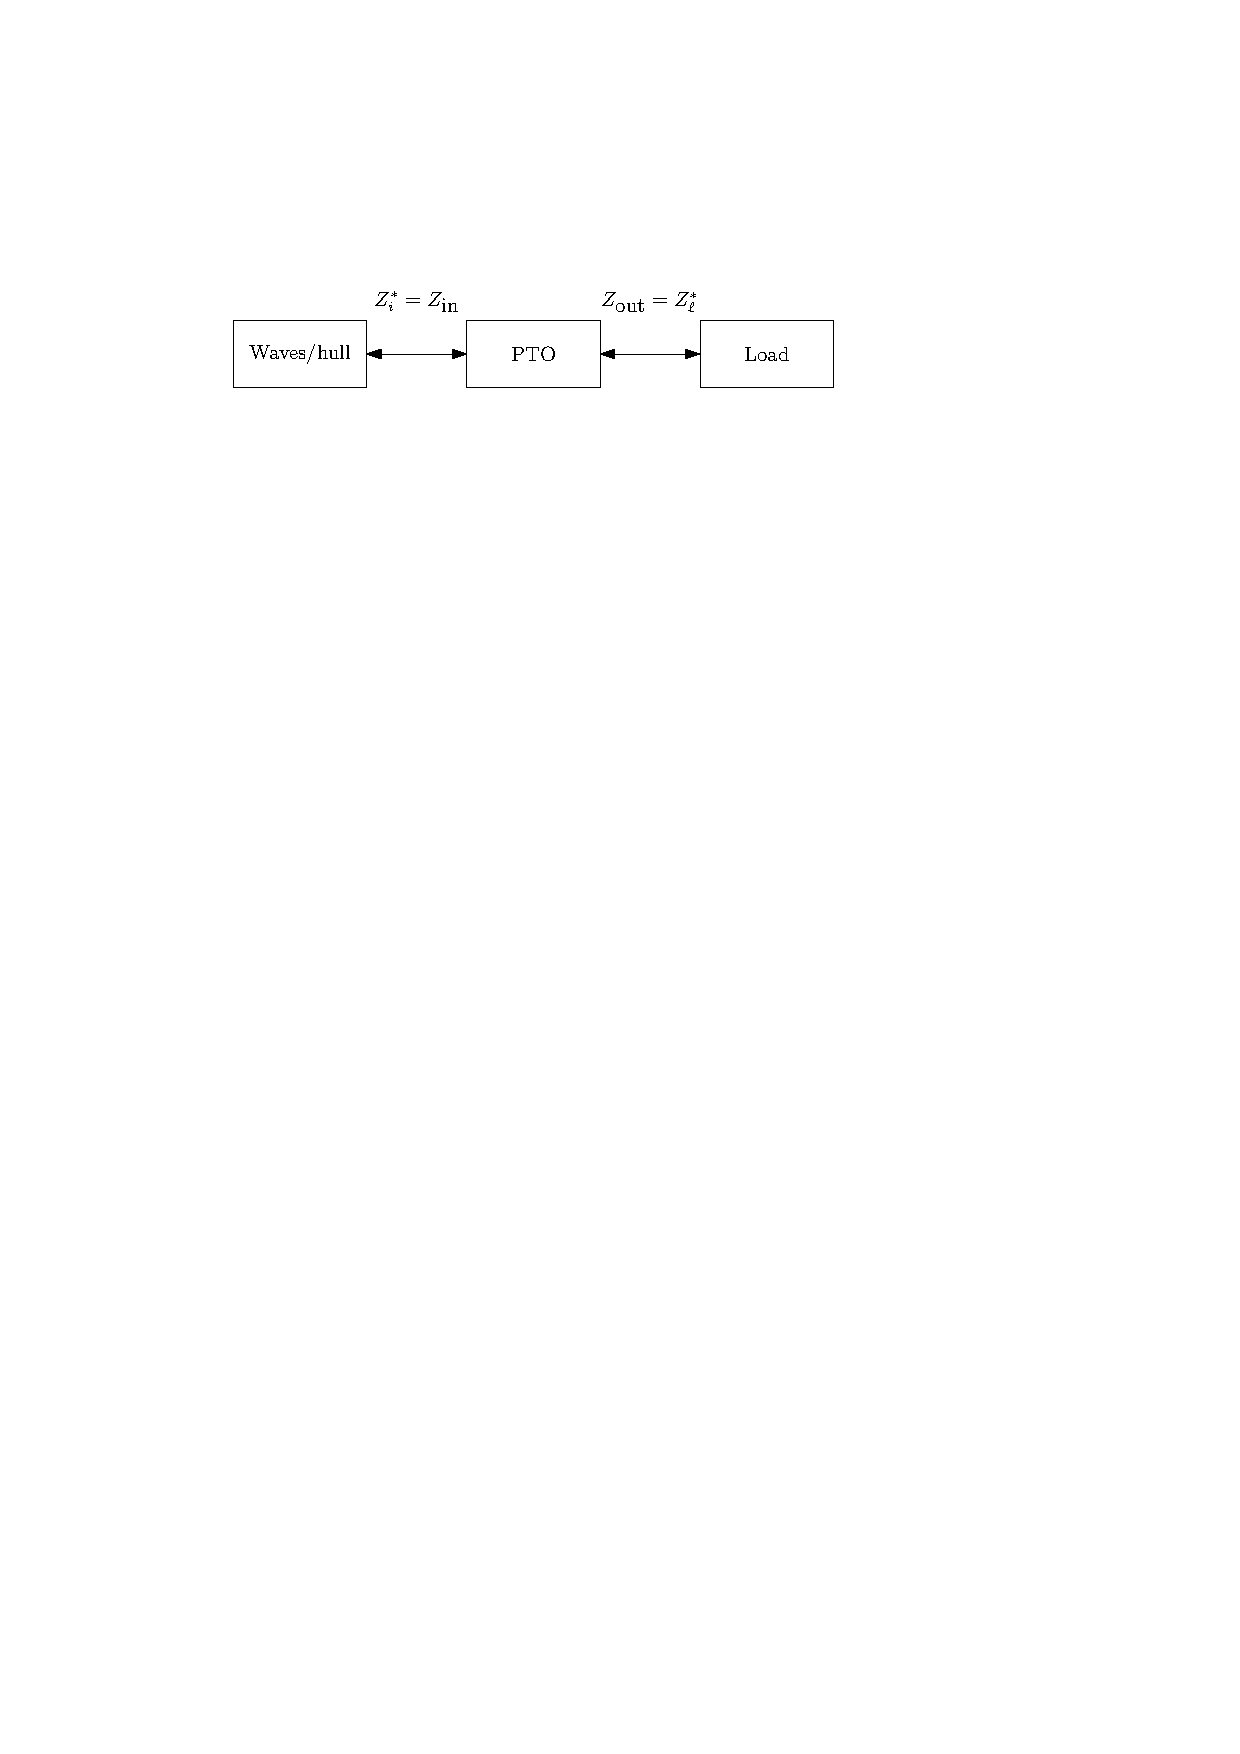
\includegraphics[width=1\columnwidth]{wec_as_multiport_power_transfer_stages.pdf}
        \caption{WEC power flow stages with impedance matching conditions.}
        \label{fig:wec_as_multiport_power_transfer_stages}
\end{figure}

Power delivered to the load is affected by both losses and reflections in the WEC system.
These two effects are distinct and must be addressed with an appreciation as such.
Losses are due to friction or electrical resistance -- this effect is often more intuitive and will not be discussed here in detail.
Reflections are due to a mismatch in the system impedances -- this effect is generally underappreciated and is the main focus of this paper.
%%% Dom feels this is a bit of an over-simplification maybe better suited for a discussion section later on. While minimizing losses is important, friction and resistance are contributors to the real part of impedance and, especially in absence of other contributors (gear ratio, Kt) being called out explicitly I think this might yield confusion.

This paper will further explore concepts of bi-conjugate impedance matching in wave energy, previously raised by \cite{Bacelli:2021aa}, with the goal of generating a more practical understanding of the utility and application of this theory. 
First, a basic review of network modeling and elements is presented (Section~\ref{sec:multi_port_networks}).
Next, this framework is applied to a WEC and used to formulate the bi-conjugate impedance matching condition (Section~\ref{sec:modeling_a_direct_drive_wec}).
This framework is then applied in a number of illustrative case studies (Section~\ref{sec:illustrative_examples}).

% ------------------------------------------------------------------
\section{Multi-port networks}\label{sec:multi_port_networks}
The multi-port network models popular in electronics and microwave systems~\cite{Marrocco:2008aa,CircuitFundamental} provide a useful construct for analyzing a WEC.
Given that these models are not currently used broadly within the wave energy field, we will now review the fundamental concepts of multi-port network models.
\figurename~\ref{fig:wec_as_multiport_transformer_gyrator} provides a central reference for this discussion, with columns pertaining to different network model elements and representations/explanations of those elements shown in each row.
First, let us consider one-port elements, which, as shown on the left hand side of \figurename~\ref{fig:wec_as_multiport_transformer_gyrator}, relate a single effort variable ($e$) to a single flow variable ($q$) through an impedance ($Z$).

\begin{figure*}
	\centering
	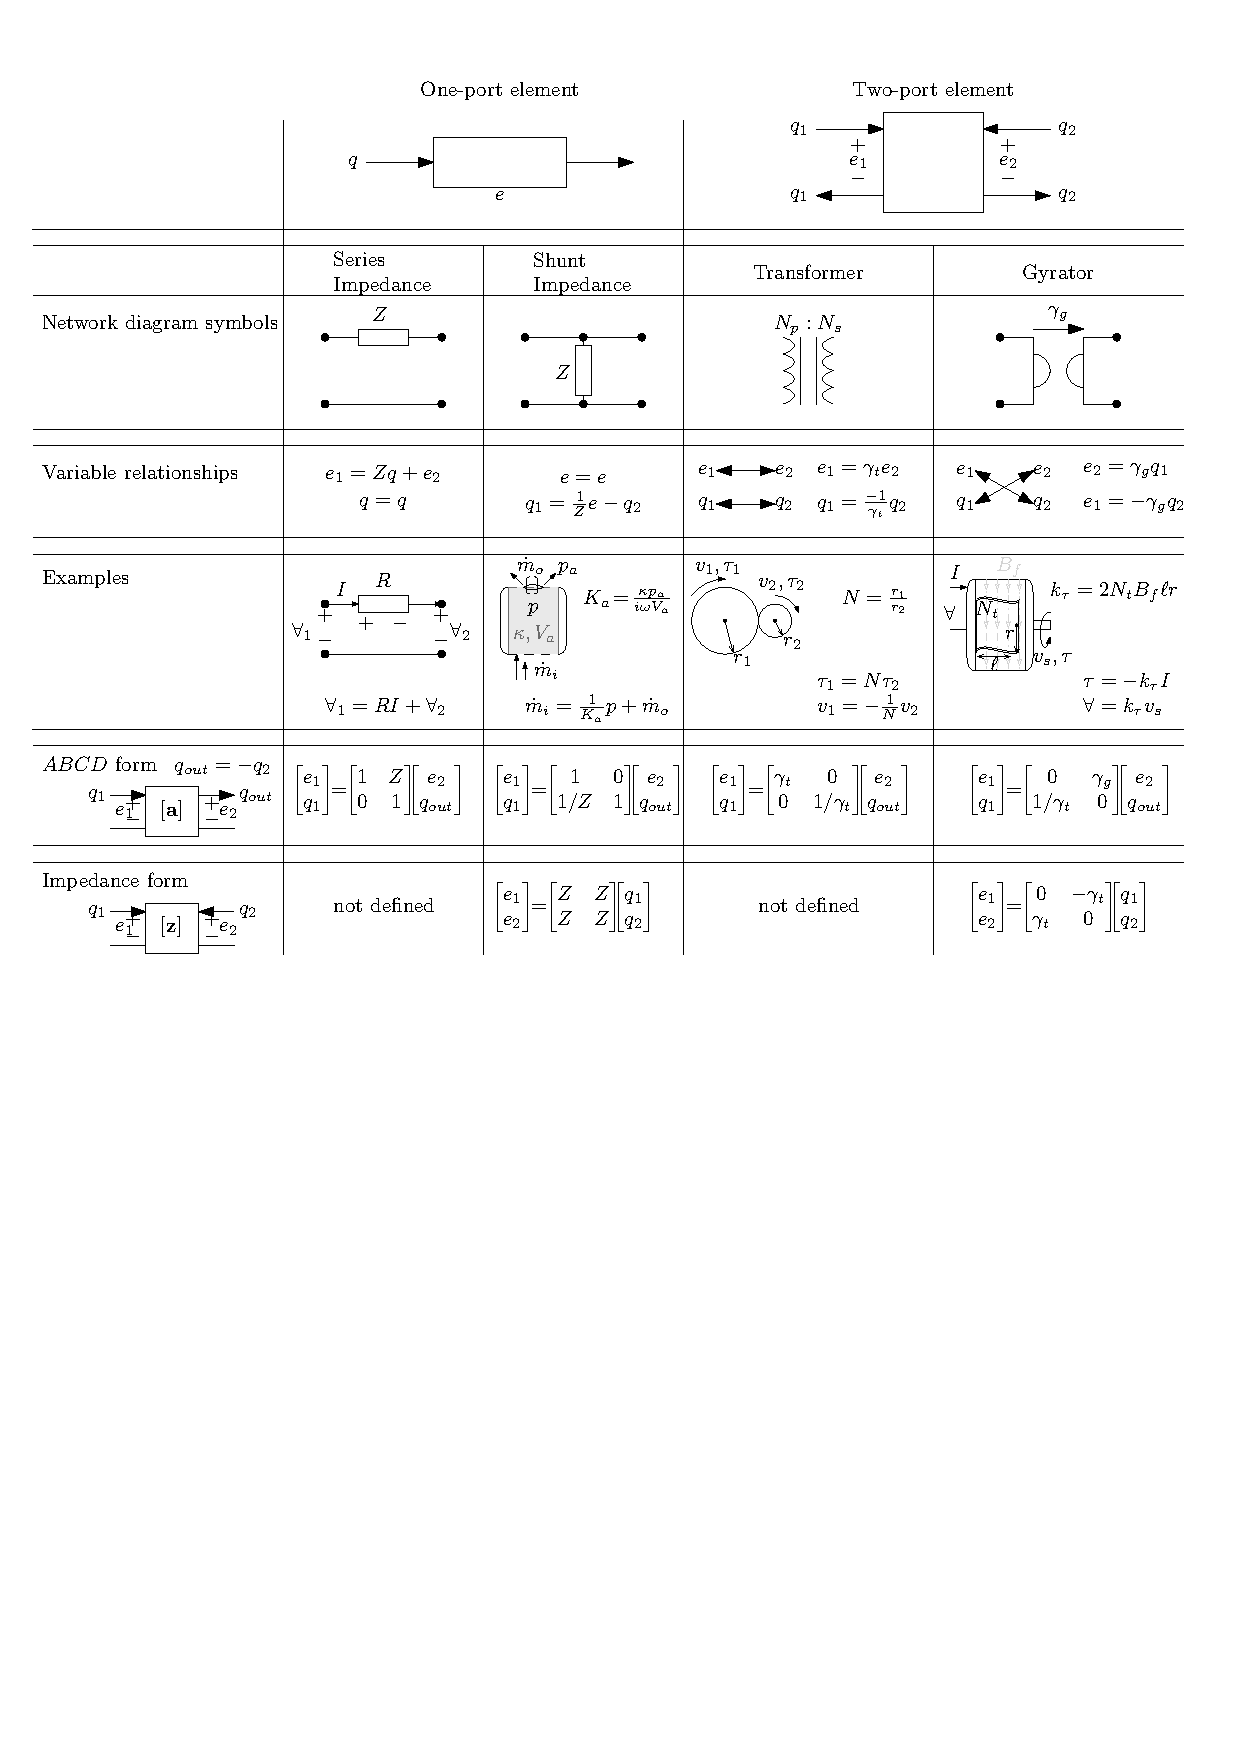
\includegraphics[width=\textwidth]{wec_as_multiport_transformer_gyrator_impedance_Z_A.pdf}
	\caption{General one- and two-port elements definition showing effort ($e$) and flow ($q$) at each port with diagrams and mathematical relationships for impedances, transformers, and gyrators.}
	% \rc{XX-add impedance in parallel} \rc{XX-can we draw the variable relationship arrows for impedances}
	\label{fig:wec_as_multiport_transformer_gyrator}
\end{figure*}

%
\begin{equation}
        Z = \frac{e}{q}
\end{equation}
%
Similarly, two-port elements relate two pairs of effort and flow variables (see the right hand side of \figurename~\ref{fig:wec_as_multiport_transformer_gyrator}).\footnote{As the ``multi-port'' name suggests, elements with more than two ports (three, four, etc.) may also be considered.}
%
\begin{equation} \label{eq:Z_mat_def_general}
        \begin{bmatrix} e_1 \\ e_2 \end{bmatrix} = \begin{bmatrix} Z_{11} & Z_{12} \\ Z_{21} & Z_{22} \end{bmatrix} \begin{bmatrix} q_1 \\ q_2 \end{bmatrix},
\end{equation}
%
The elements of any two-port impedance matrix may be defined as follows \cite{CircuitFundamental}.
%
\begin{equation} \label{eq:Z_mat_elements_def}
        \begin{aligned}
                Z_{11}& = \frac{e_1}{q_1} \bigg \vert_{q_2=0} \quad
                Z_{12} = \frac{e_1}{q_2} \bigg \vert_{q_1=0}  \\[1em]
                Z_{21}& = \frac{e_2}{q_1} \bigg \vert_{q_2=0} \quad
                Z_{22} = \frac{e_2}{q_2} \bigg \vert_{q_1=0} 
        \end{aligned}
\end{equation}
%
The product of the effort and flow variables on each port is power.
Note also the sign conventions illustrated in \figurename~\ref{fig:wec_as_multiport_transformer_gyrator}, which result in power flow into the two-port network from both sides, summing to zero for a lossless system.
%
In addition to the ``impedance form'' shown in \eqref{eq:Z_mat_def_general}, there are many equivalent formulations for modeling two-port networks~\cite{CircuitFundamental}.
Certain formulations may be easier to work with depending on the task at hand.
In this paper, we will also utilize the ``$ABCD$ form'' (also sometimes referred to as ``chain,'' ``cascade,'' or ``transmission'' form):
%
\begin{equation}
        \label{eq:abcd_mat_def_general}
        \begin{bmatrix} e_1 \\ q_1 \end{bmatrix}
        = 
        \begin{bmatrix} A & B \\ C & D \end{bmatrix}
        \begin{bmatrix} e_2 \\ - q_2 \end{bmatrix},
\end{equation}
%
Similarly to \eqref{eq:Z_mat_elements_def}, the elements of the $ABCD$ matrix are defined as follows.
%
\begin{subequations} \label{eq:abcd_mat_elements_def}
        \begin{align}
                A &= \frac{e_1}{e_2} \bigg \vert_{q_2=0}  \quad
                B = - \frac{e_1}{q_2} \bigg \vert_{e_2=0}  \\[1em]
                C &= \frac{q_1}{e_2} \bigg \vert_{q_2=0}  \quad
                D = - \frac{q_1}{q_2} \bigg \vert_{e_2=0} 
        \end{align}
\end{subequations}
%
Note that the impedance form and $ABCD$ form matrix elements are explicitly interrelated (see, e.g., \cite{CircuitFundamental}).
For example, we may relate the impedance matrix and $ABCD$ as
%
\begin{equation}
        \begin{bmatrix}
                Z_{11} & Z_{12} \\ Z_{21} & Z_{22}
        \end{bmatrix}
        =
        \frac{1}{C}
        \begin{bmatrix}
                A & \Delta \left[ \mathbf{a} \right] \\ 1 & D
        \end{bmatrix},
\label{eq:abcd_to_Z}
\end{equation}
%
where $\Delta \left[ \mathbf{a} \right]$ is the determinant of the $ABCD$ matrix.
From \eqref{eq:abcd_to_Z}, we can see that some representations may be undefined for certain two-port elements (e.g., if $C=0$ in the $ABCD$ form, the impedance form will be undefined).
%
An important property of a two-port element is that it can be collapsed into a one-port element if one of the ports is terminated with a load and has no independent sources. 
Whereas the general two-port element has four variables, two of which are independent, in the scenario where one port is terminated with a load, the system loses a degree of freedom. 
Thus, in this case, we may simplify the system as a one-port element (i.e., a single impedance). 
With these general properties in hand, let us now consider some fundamental multi-port elements shown in \figurename~\ref{fig:wec_as_multiport_transformer_gyrator}.

% ------------------------------------------------------------------
\subsection{Impedances (one-ports)}\label{sec:impedances}
To incorporate dynamics and losses into the system description, we utilize one-port impedance elements, which describe how components impede flow by opposing effort. 
In general, for a series impedance in a closed loop (see ``series impedance'' in \figurename~\ref{fig:wec_as_multiport_transformer_gyrator}), we may write,
%
\begin{subequations}
        \begin{align}
                e_1 &= Zq_1 + e_2 \\
                q_1 &= -q_2 ,
        \end{align}
        \label{eq:impedance_eom}%
\end{subequations}
%
which can be equivalently represented in $ABCD$ form as,
%
\begin{equation}
        \begin{bmatrix}
                e_1 \\ q_1
        \end{bmatrix}
        =
        \begin{bmatrix}
                1 & Z \\ 0 & 1
        \end{bmatrix}
        \begin{bmatrix}
                e_2 \\ - q_2
        \end{bmatrix} .
        \label{eq:impedance_abcd}%
\end{equation}
%
Alternatively, if the impedance is connected in parallel (see ``shunt impedance'' in \figurename~\ref{fig:wec_as_multiport_transformer_gyrator}), we may write
%
\begin{subequations}
        \begin{align}
                e_1 &=  e_2 \\
                q_1 &= \frac{1}{Z} e_2 - q_2 ,
        \end{align}
        \label{eq:parallel_impedance_eom}%
\end{subequations}
%
which can be equivalently represented in $ABCD$ form as,
%
\begin{equation}
        \begin{bmatrix}
                e_1 \\ q_1
        \end{bmatrix}
        =
        \begin{bmatrix}
                1 & 0 \\ \frac{1}{Z} & 1
        \end{bmatrix}
        \begin{bmatrix}
                e_2 \\ - q_2
        \end{bmatrix} .
        \label{eq:parallel_impedance_abcd}%
\end{equation}

% ------------------------------------------------------------------
\subsection{Transformers}\label{sec:trasnformers}
Electric transformers are widely known and understood to convert between different voltage levels.
For an ideal transformer, we may define a constant $\gamma_{t}$ that relates the effort and flow variables (see \figurename~\ref{fig:wec_as_multiport_transformer_gyrator}).
%
\begin{subequations}
        \begin{align}
               e_1 &= \gamma_{t} e_2 \\
               q_1 &= -\frac{1}{\gamma_t} q_2
        \end{align}
        \label{eq:transformer_eom}%
\end{subequations}
%
Note that, as shown in \figurename~\ref{fig:wec_as_multiport_transformer_gyrator}, \eqref{eq:transformer_eom} relates the flow at port 1 to the flow at port 2 and effort at port 1 to the effort at port 2 (i.e., the flows are directly related to each other, as are the efforts).
In an electric transformer, the constant $\gamma_t$ is the ratio of windings on its primary and secondary sides ($\gamma_t=N_p/N_s$).
A geared transmission is a mechanical example of a transformer (see \figurename~\ref{fig:wec_as_multiport_transformer_gyrator}); in this case, $\gamma_{t}$ is the gear ratio.
In $ABCD$ form, we may represent a transformer as
%
\begin{equation}
        \begin{bmatrix}
                e_1 \\ q_1
        \end{bmatrix}
        =
        \begin{bmatrix}
                \gamma_{t} & 0 \\ 0 & 1/\gamma_{t}
        \end{bmatrix}
        \begin{bmatrix}
                e_2 \\ - q_2
        \end{bmatrix} .
        \label{eq:transformer_abcd}
\end{equation}
%
Recalling \eqref{eq:abcd_to_Z}, we may see that the impedance form representation for a transformer is not defined ($1/C \rightarrow \infty$).

% ------------------------------------------------------------------
\subsection{Gyrators}\label{sec:gyrators}
Gyrators are effectively the opposites of transformers in that they relate the flow at one port to the effort at the other port (see \figurename~\ref{fig:wec_as_multiport_transformer_gyrator}).
In general, we may write
%
\begin{subequations}
        \begin{align}
               e_1 &= - \gamma_g q_2 \\
               q_1 &= \frac{1}{\gamma_g} e_2 ,
        \end{align}
        \label{eq:gyrator_eom}%
\end{subequations}
%
where $\gamma_g$ is the gyration modulus.
In $ABCD$ form, a gyrator can be represented as
%
\begin{equation}
        \begin{bmatrix}
                e_1 \\ q_1
        \end{bmatrix}
        =
        \begin{bmatrix}
                0 & \gamma_g \\ 1/\gamma_g & 0
        \end{bmatrix}
        \begin{bmatrix}
                e_2 \\ - q_2
        \end{bmatrix} .
        \label{eq:gyrator_abcd}
\end{equation}
%
An electric motor/generator is a very relevant example of a gyrator.
In that case, the gyration modulus is the motor constant ($\gamma_g=k_\tau$).
The direction of the arrow in a gyrator schematic as shown in \figurename~\ref{fig:wec_as_multiport_transformer_gyrator} indicates the directionality of the element: the \emph{positive} product of the flow at the arrow's tail with the gyration modulus gives the effort at the arrow's head ($e_2 = \gamma_g q_1$ as drawn in \figurename~\ref{fig:wec_as_multiport_transformer_gyrator} with the arrow pointing from port 1 to port 2) and the effort at the arrow's tail is the \emph{negative} product of the gyration modulus and effort at the head ($e_1= - \gamma_g q_2$ as drawn in \figurename~\ref{fig:wec_as_multiport_transformer_gyrator}).
Note that a cascade of two gyrators has the composite effect of a transformer.
For example, two lossless electric motor/generators with coupled shafts would be equivalent to an electrical transformer with a winding ratio of $\gamma_t=N_p/N_s=\gamma_{g1}/\gamma_{g2}$.

% ------------------------------------------------------------------
\section{Modeling a direct drive WEC}\label{sec:modeling_a_direct_drive_wec}
Using the general definitions for network diagram modeling presented in Section~\ref{sec:multi_port_networks}, we now wish to model a WEC.
To this end, let us consider the heaving buoy style ``WaveBot'' device with a direct drive PTO as shown in \figurename~\ref{fig:wec_as_multiport_physical_diagram} \cite{Forbush:2024aa}.
Table~\ref{tab:wec_physical_params} lists key parameters for the WaveBot.
We will first present the WEC and its governing equations in further detail (Section~\ref{sec:dynamic_and_kinematic_equations}) and then utilize those governing equations to represent the system via multi-port network models (Section~\ref{sec:modeling_with_a_network_diagram}).

\begin{figure}[tb]
        \centering
        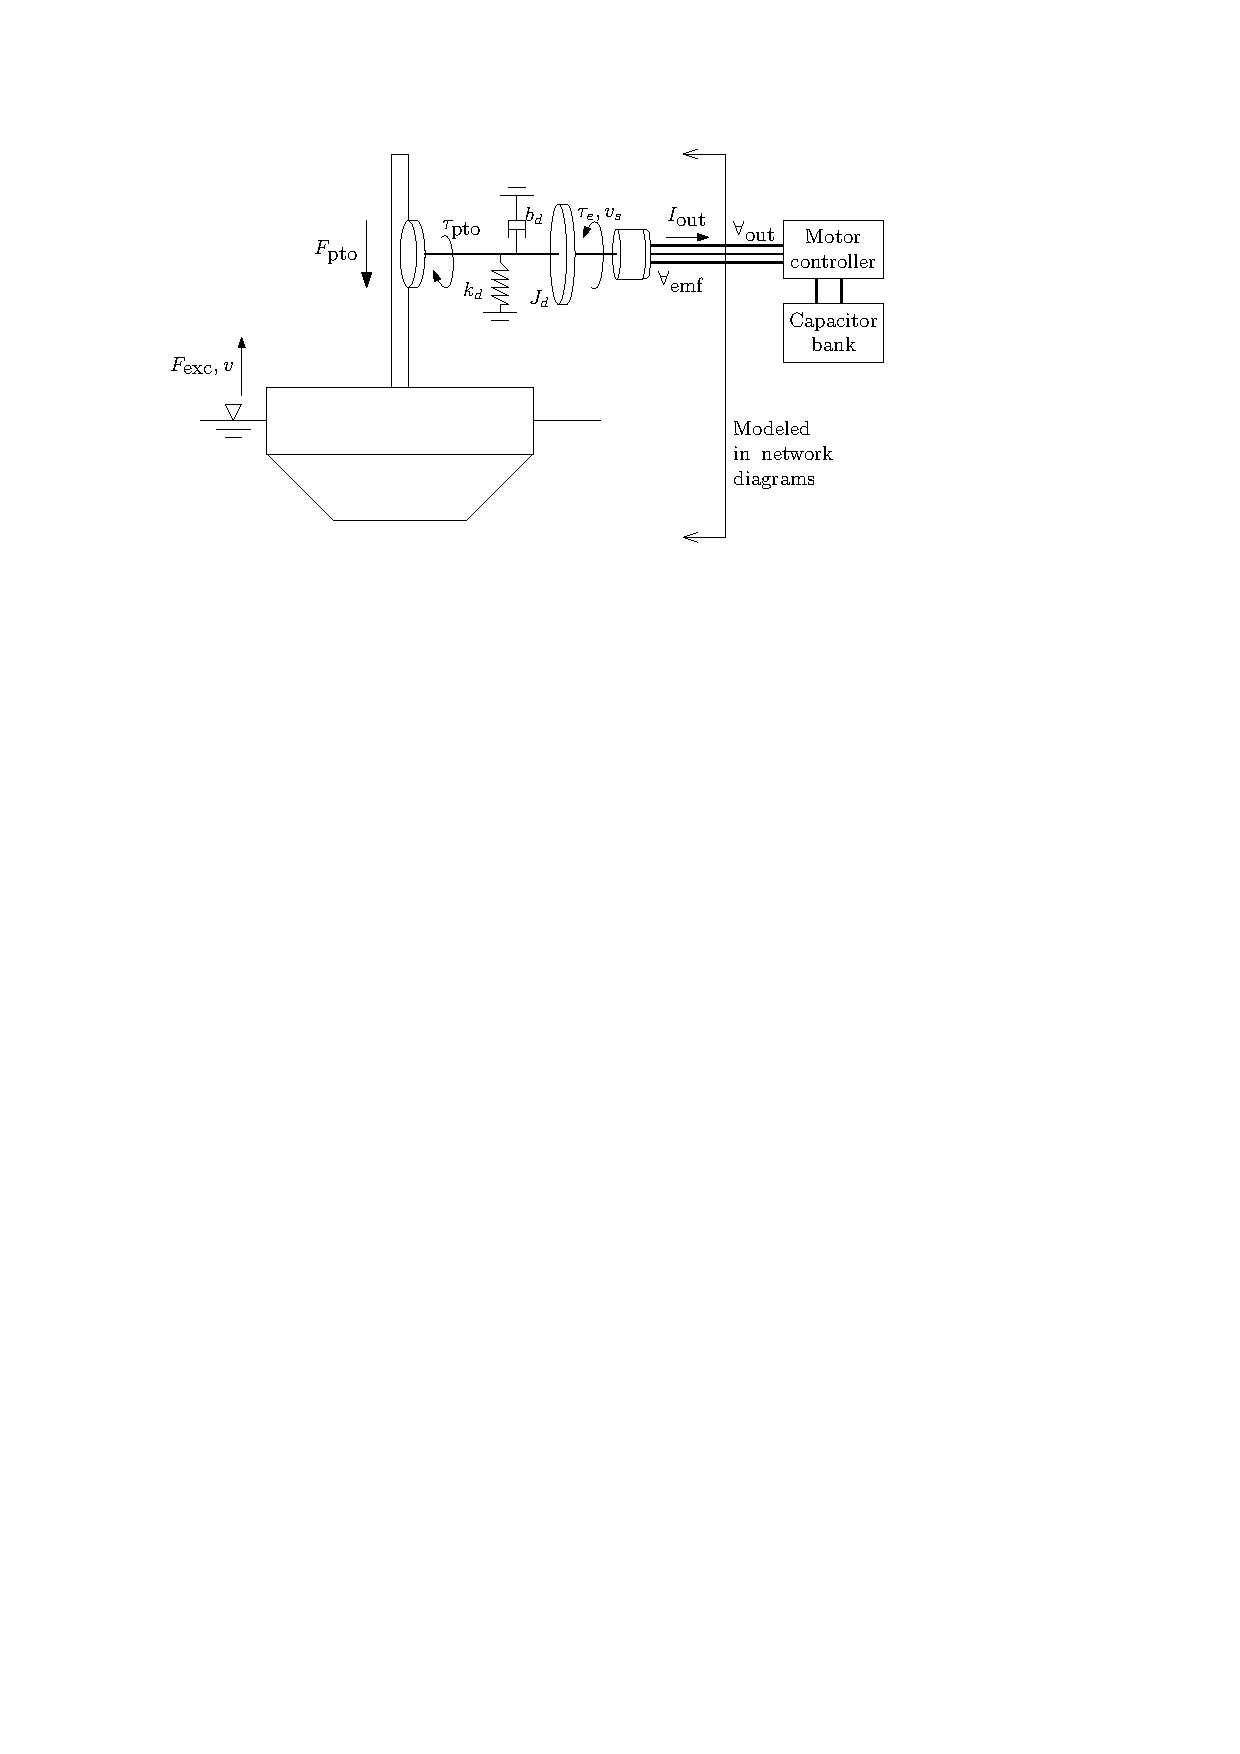
\includegraphics[width=1\columnwidth]{wec_as_multiport_phyiscal_diagram.pdf}
        \caption{WaveBot device diagram.}
        \label{fig:wec_as_multiport_physical_diagram}
\end{figure}

\begin{table}[tb]
        \caption{Key physical parameters of the WaveBot.}
        \label{tab:wec_physical_params}
        \centering

        \begin{tabular}{rc}
        \hline

        \hline
        \textbf{Parameter} & \textbf{Value} \\
        \hline
        Rigid body mass, $m$ [kg]                       & 875 \\
        Hydrostatic stiffness, $k_h$ [kN/m]             & 2.44 \\
        Linear friction coefficient, $b_f$ [Ns/m]       & 1 \\ % XX - is this reasonable?
        Linear to rotational gear ratio, $N$ [rad/m]    & 12.4666 \\
        Shaft inertia, $J_d$ [kg\,m$^2$]                & 2 \\ % XX - is this reasonable?
        Shaft friction, $b_d$ [Nm\,s/rad]               & 1 \\ % XX
        Grounded shaft spring stiffness, $k_d$ [Nm/rad] & 0 \\ % XX
        Torque constant, $k_\tau$ [Nm/A]                & 6.1745 \\
        Motor winding resistance, $R_w$ [$\Omega$]      & 0.5 \\
        Motor winding inductance, $L_w$ [H]             & 0 \\
        \hline

        \hline
        \end{tabular}
\end{table}

% ------------------------------------------------------------------
\subsection{Dynamic and kinematic equations}\label{sec:dynamic_and_kinematic_equations}
Vertical motion of the buoy can be expressed as a dynamic equation dependent on the PTO force\footnote{Note that we define the ``PTO'' force in the opposite direction of the excitation force and velocity as shown in \figurename~\ref{fig:wec_as_multiport_physical_diagram}. This sign convention, where, as in \eqref{eq:eom_rectilinear_motion}, we have an expression of the form $Z q = e_1 - e_2$, is most common in network diagrams and control engineering and therefore used herein.} ($F_{\textrm{pto}}$), the excitation force ($F_{\textrm{exc}}$), and the intrinsic impedance ($Z_i$) \cite{Falnes:2002aa}.
%
\begin{subequations}
\begin{gather}
        F_{\textrm{exc}} - F_{\textrm{pto}} = Z_i v \label{eq:eom_rectilinear_motion} \\
        Z_i(\omega) = B(\omega) + b_f + j \left( \omega \left( m + A(\omega) \right) - \frac{k_{h}}{\omega}\right)
\end{gather}
\end{subequations}
%
\noindent{}Here, $A(\omega)$ is the added mass, $B(\omega)$ is the radiation damping, $k_h$ is the hydrostatic stiffness, $b_f$ accounts for linear friction effects, and $m$ is the rigid body inertia.
The imaginary unit is $j$ and $\omega$ is the angular frequency.
A block diagram\footnote{\label{fn:block_diagrams}Note that block diagrams are related to but distinct from the network diagrams used elsewhere in this paper. To emphasize this distinction, a grey fill is used for blocks in \figurename~\ref{fig:wec_as_multiport_block_diagram}.} in \figurename~\ref{fig:wec_as_multiport_block_diagram} shows the system described by \eqref{eq:eom_rectilinear_motion}.
In \figurename~\ref{fig:wec_as_multiport_block_diagram}, the PTO force is determined based on the PTO input impedance ($Z_{\textrm{in}}$) -- the details of this will be discussed in more detail in Section~\ref{sec:pto_input_and_output_impedances}; the excitation force ($F_{\textrm{exc}}$) is determined from the excitation transfer function ($H_{\textrm{exc}}$) based on the wave elevation~($\eta$).

\begin{figure}[tb]
        \centering
        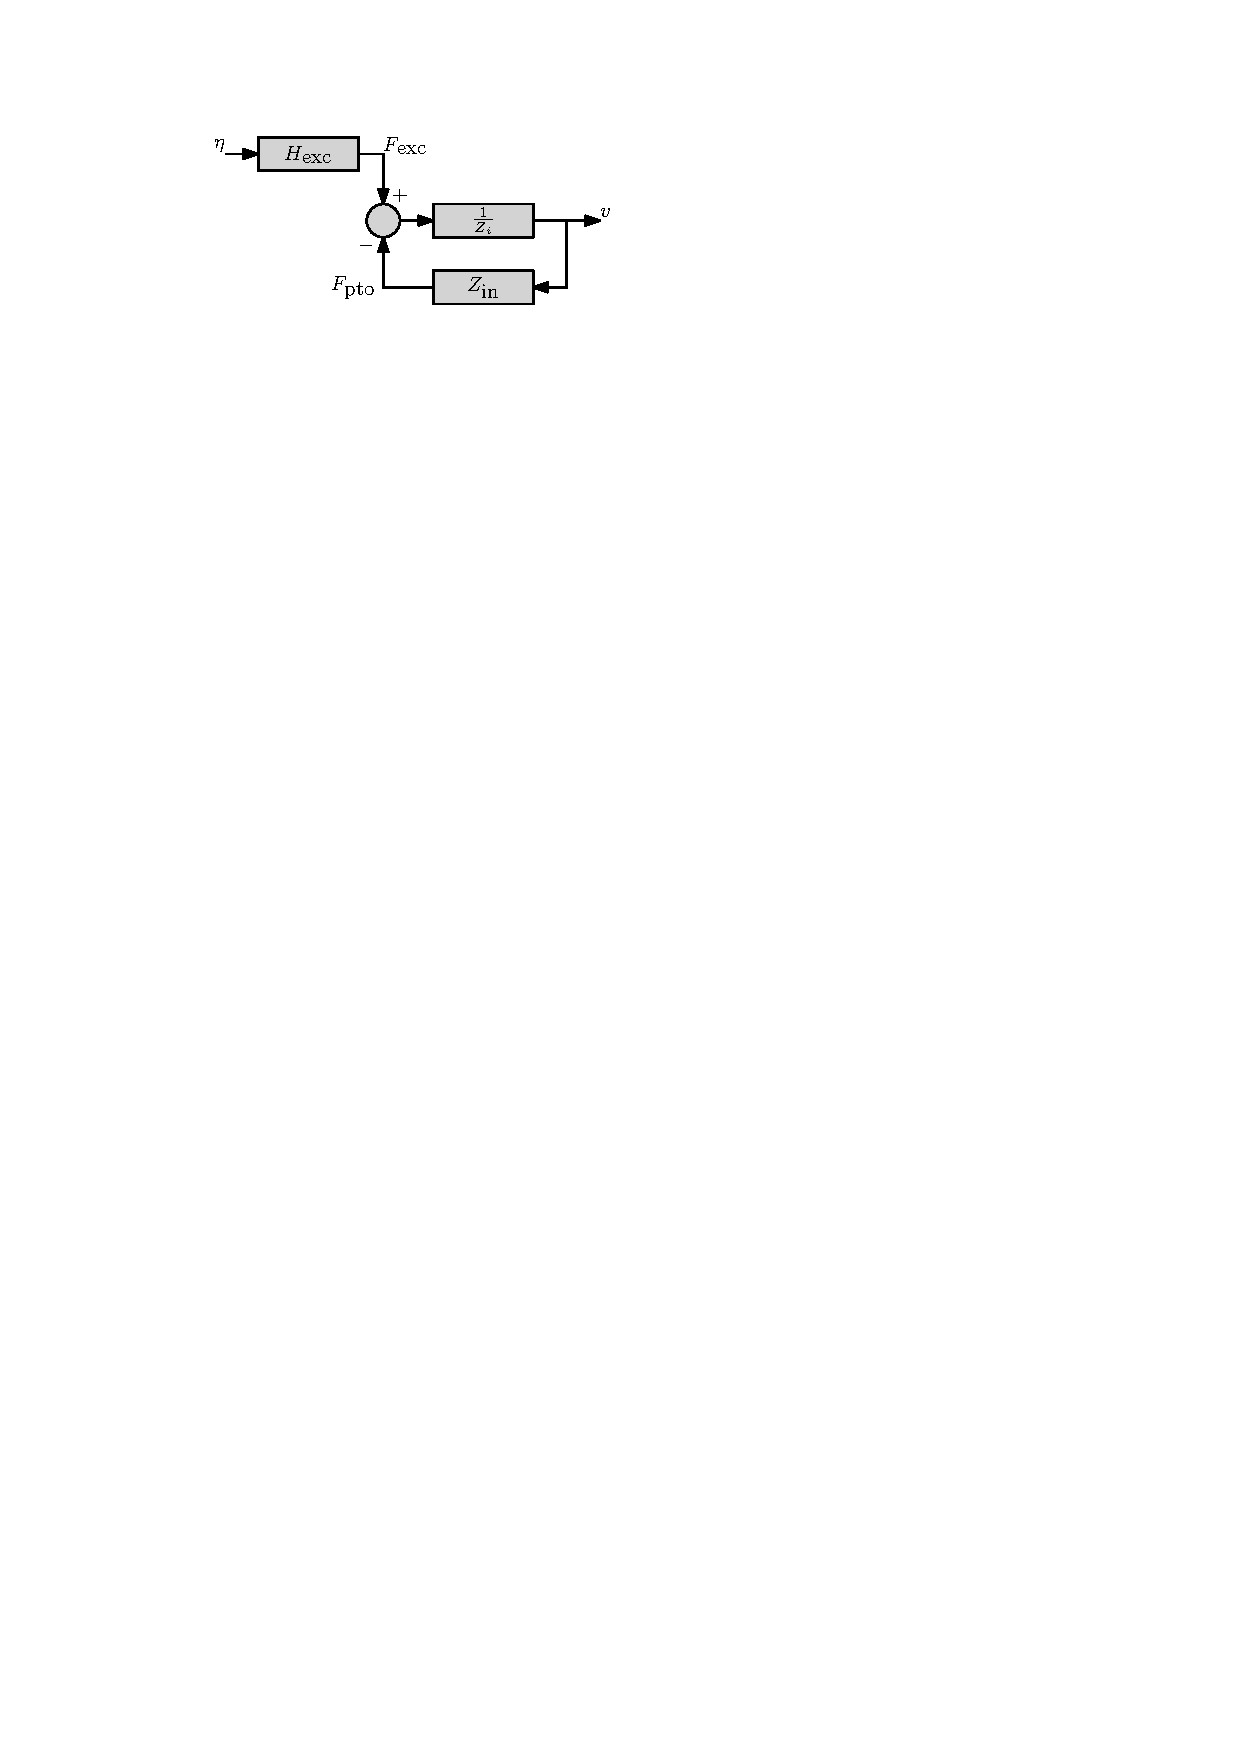
\includegraphics[width=0.8\columnwidth]{wec_as_multiport_block_diagram.pdf}
        \caption{Generic block diagram for a wave energy converter.}
        \label{fig:wec_as_multiport_block_diagram}
\end{figure}

The rectilinear vertical velocity ($v$) and force ($F_{\textrm{pto}}$) in \eqref{eq:eom_rectilinear_motion} are transformed into rotational velocity ($v_s$) and torque ($\tau_{\textrm{pto}}$) on a rotating shaft by a ``rack and pinion'' style mechanism with radius $N$.
%
\begin{subequations}
        \begin{gather}
                v_s = N v \\
                \tau_{\textrm{pto}} = \frac{1}{N} F_{\textrm{pto}}
        \end{gather}
        \label{eq:rack_and_pinion_transmission}%
\end{subequations}
%
Comparing \eqref{eq:rack_and_pinion_transmission} and \eqref{eq:transformer_eom}, we may note that the rack and pinion is an example of a transformer.

The rotating drive-train shaft has characteristic linear friction ($b_d$), inertia ($J_d$), and may include some non-zero spring stiffness effect against the ground ($k_d$).
The opposite end of the drive-train shaft interfaces with an electric motor/generator that produces an electromagnetic torque ($\tau_e$).
Thus, we may describe the drive-train dynamics as follows.
%
\begin{subequations}
        \begin{gather}
                \tau_{\textrm{pto}} - \tau_e = Z_d v_s \\
                % Z_d = i \omega J_d + b_d + \frac{k_d}{i \omega}
                Z_d = b_d + j \left( \omega J_d - \frac{k_d}{\omega} \right)
        \end{gather}
\end{subequations}

The electric motor/generator can be considered to have the composite characteristics of a pure gyrator and an impedance.
For the gyrator element, the machine has a characteristic torque constant (gyration modulus) $k_\tau$ that relates back EMF voltage ($\forall_{\textrm{emf}}$) to shaft speed and electromagnetic torque to the quadrature current ($I_{\textrm{out}}$) when using a Park power invariant transformation.
%
\begin{subequations}
        \begin{gather}
                v_s = \frac{1}{k_\tau}\forall_{\textrm{emf}} \\
                \tau_e = k_\tau I_{\textrm{out}}
        \end{gather}
\end{subequations}
%
In addition to its gyration effect, the motor has a characteristic impedance ($Z_w$) that captures the effects of winding resistance ($R_w$) and inductance ($L_w$), and relates the output current to the back EMF voltage ($\forall_{\textrm{emf}}$) and output voltage ($\forall_{\textrm{out}}$).
% \rc{-XX reference figure 6b?}
%
\begin{subequations}
        \begin{gather}
                \forall_{\textrm{emf}} - \forall_{\textrm{out}} = Z_w I_{\textrm{out}}\\
                Z_w = R_w + j \omega L_w \label{eq:winding_impedance}
        \end{gather}
\end{subequations}

Finally, we may define a load impedance ($Z_\ell$) that represents how current is modulated by the motor controller relative to voltage.
%
\begin{equation}
        Z_\ell = \frac{\forall_{\textrm{out}}}{I_{\textrm{out}}}
        \label{eq:load_impedance}
\end{equation}
%
In practice, the load impedance will be defined by a controller ($C$).
It is generally convenient to implement a feedback controller that commands motor current based on the angular velocity ($I_{\textrm{out}}$ and $v_s$, respectively, in \figurename~\ref{fig:wec_as_multiport_physical_diagram}).
%
\begin{subequations}
\begin{gather}
        I_{\textrm{out}} = C v_s \\  
        Z_\ell = \frac{1}{C} k_\tau - Z_w     
\end{gather}
\end{subequations}
%
While many forms may be used for $C$, a simple proportional-integral (PI) structure can be quite effective \cite{Coe2020a}.
%
\begin{equation}
        C_{PI} = k_p + \frac{1}{j \omega} k_i 
        \label{eq:pi_controller_structure}
\end{equation}
%
The current command in \eqref{eq:pi_controller_structure} is thus defined as the sum of products \emph{proportional} to velocity ($v_s k_p$) and the \emph{integral} of velocity ($\frac{v_s}{j \omega} k_i$, i.e., position).

% ------------------------------------------------------------------
\subsection{Modeling with a network diagram}\label{sec:modeling_with_a_network_diagram}

The WaveBot device shown in \figurename~\ref{fig:wec_as_multiport_physical_diagram} and described in Section~\ref{sec:dynamic_and_kinematic_equations} can be represented with network diagrams as shown in \figurename~\ref{fig:wec_as_multiport_circuits}.
Various levels of abstraction/detail can be achieved in this style of diagram.
\figurename~\ref{fig:wec_as_multiport_circuits}a shows the highest level of detail, whereas \figurename~\ref{fig:wec_as_multiport_circuits}b and \figurename~\ref{fig:wec_as_multiport_circuits}c increasingly combine elements to achieve a single two-port network to represent the PTO.
We will return to \figurename~\ref{fig:wec_as_multiport_circuits}d-f for later discussion.

\begin{figure}[htbp]
        \centering
        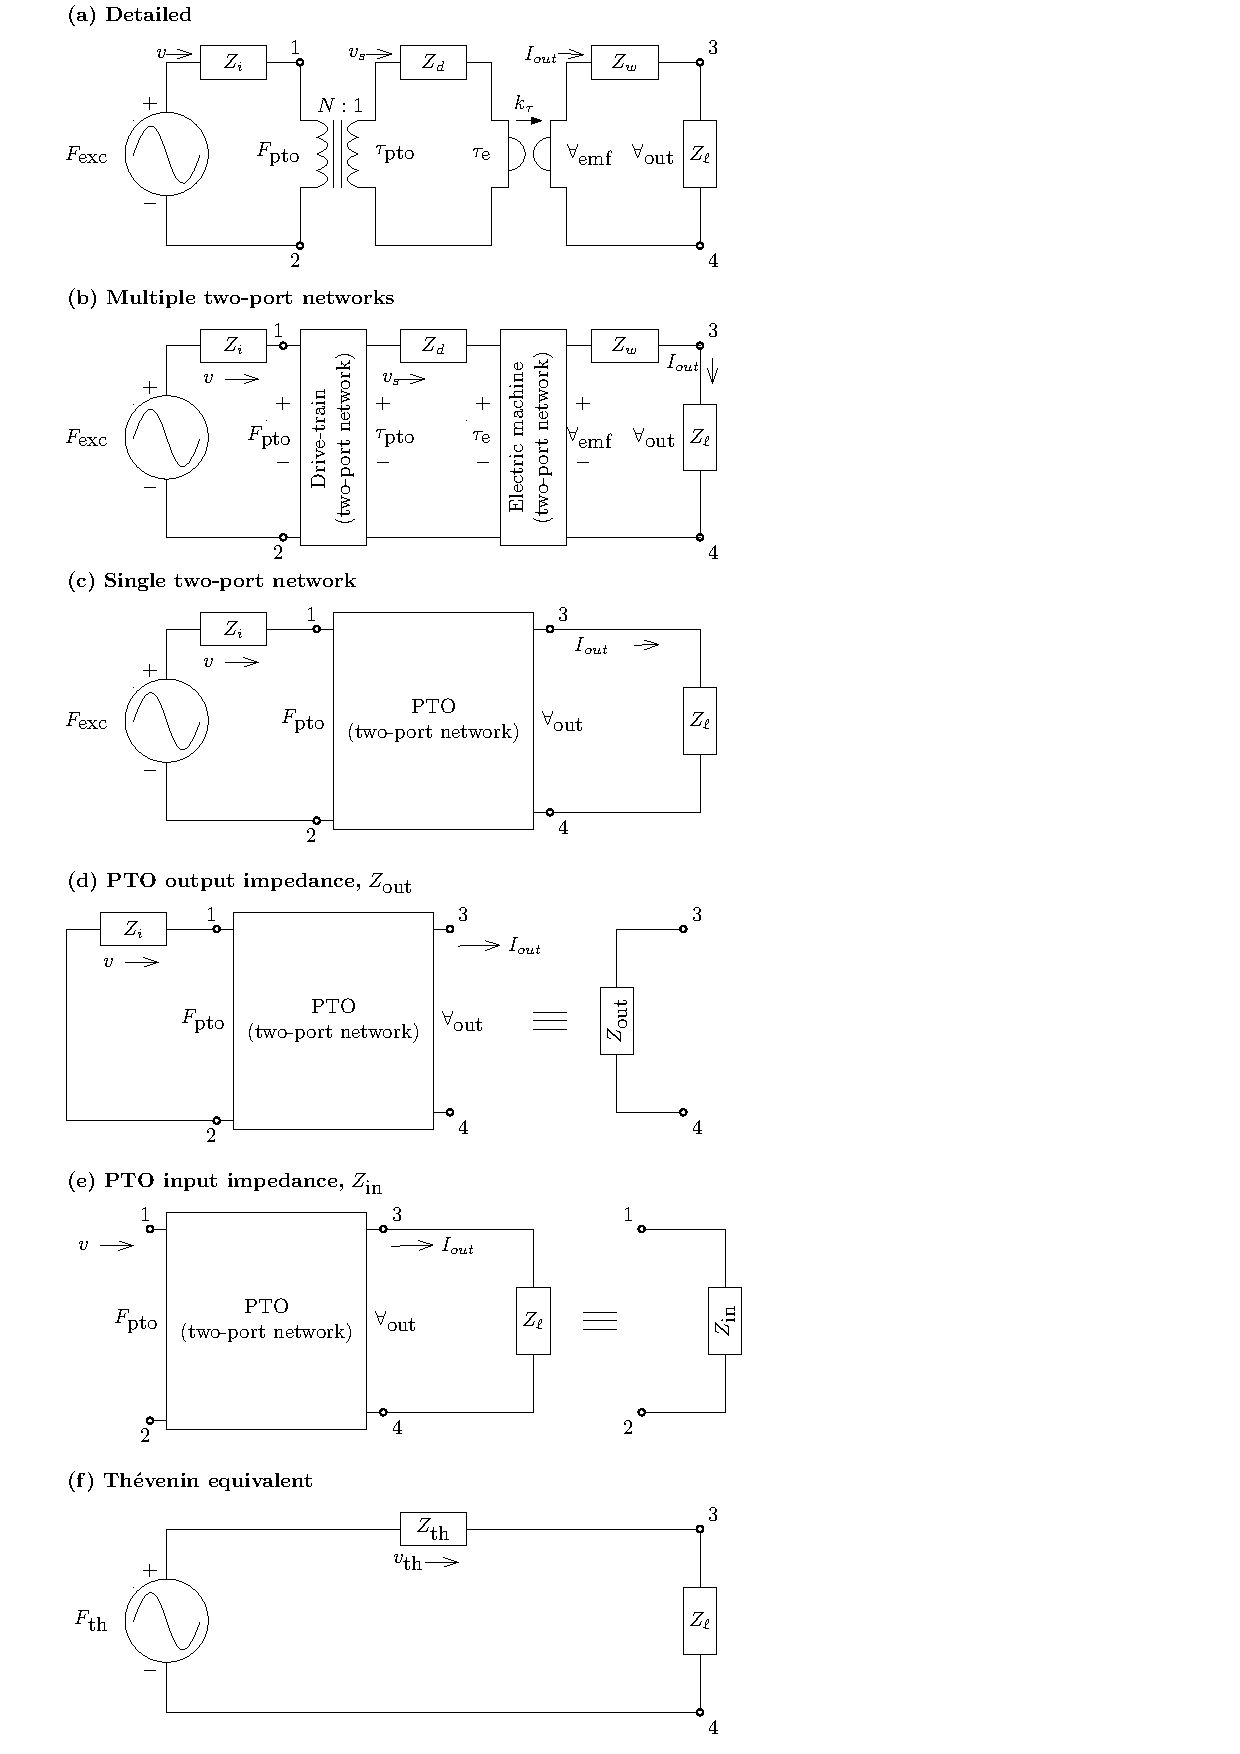
\includegraphics[width=1\columnwidth]{wec_as_multiport_circuits.pdf}
        \caption{Circuit diagrams representing a wave energy converter. Points 1, 2, 3, and 4 are consistent throughout the different diagrams.}
        \label{fig:wec_as_multiport_circuits}
\end{figure}

Throughout literature, there are many different sign conventions utilized for multi-port systems. 
In \figurename~\ref{fig:wec_as_multiport_circuits}a, we defined $v_s$ and $I_{\textrm{out}}$ as vectors leaving the two-port elements, rather than entering. 
This convention is beneficial in two ways:
\begin{itemize}
         \item This convention allows for consistency when cascading two-ports. 
         With $q_{\textrm{out}} = -q_2$ in \eqref{eq:Z_mat_def_general} being positive out, we may ensure that the direction of the flow variable out of one cascaded stage (as it appears in the transmission matrix) is equal to the flow into the next stage. 
         This is shown in \eqref{eq:abcd_mat_def_general}, where the flow variables $q_1$ and $q_{\textrm{out}} = -q_2$ have the same power flow direction.
         %
         \item The power industry customarily to considers the flow variable $q_2$ as leaving the two-port. 
         Flow entering through the positive polarity of an element implies that the element is absorbing power~\cite{CircuitFundamental} -- this is known as the \textit{passive sign convention}.
         With the current $I_{\textrm{out}}$ flowing into the positive terminal of $\forall_{\textrm{out}}$, the load $Z_\ell$ absorbs power when power is positive.
\end{itemize}
Yet, to follow the convention for standard two-port networks, we define the flow variables $q$ as vectors entering both sides of the two-port, as shown in \figurename~\ref{fig:wec_as_multiport_transformer_gyrator} and \eqref{eq:Z_mat_def_general}. 
This means that $I_{\textrm{in}} = -I_{\textrm{out}}$, with the minus sign accounting for the opposite senses of the two currents. 
As a result, the impedance matrix and the transmission matrix follow the formulas found in most textbooks. 
This allows us to directly adopt well-known input and output impedance formulas, methods to convert between impedance and transmission form, and other techniques for performing design analysis.

We now consider two equivalent approaches for producing multi-port models to represent our WEC.
First, we directly obtain a single two-port model for the PTO as shown in \figurename~\ref{fig:wec_as_multiport_circuits}c.
Next, we show an alternative approach of combining the cascading networks shown in \figurename~\ref{fig:wec_as_multiport_circuits}b to arrive at an equivalent result.
These multi-port models for the WEC are then used to formulate a number of expressions useful in the WEC design problem.

% ------------------------------------------------------------------
\subsubsection{PTO impedance matrix}\label{sec:pto_impedance_matrix}

For the network shown in \figurename~\ref{fig:wec_as_multiport_circuits}c, we may write an impedance matrix to describe the two-port element representing the PTO.
%
\begin{equation}
        \label{eq:Z_mat_def}
        \begin{bmatrix} 
                F_{\textrm{pto}} \\
                \forall_{\textrm{out}} 
        \end{bmatrix} 
        = 
        \begin{bmatrix} 
                Z_{11} & Z_{12} \\ 
                Z_{21} & Z_{22} 
        \end{bmatrix} 
        \begin{bmatrix} 
                v \\
                I_{\textrm{in}} 
        \end{bmatrix}.
\end{equation}
%
Utilizing \eqref{eq:Z_mat_elements_def} and the equations for our system of interest presented in Section~\ref{sec:dynamic_and_kinematic_equations}, the elements of the impedance matrix in \eqref{eq:Z_mat_def} may be written out as follows.
%
\begin{subequations}
        \begin{align}
                &Z_{11} = \frac{e_1}{q_1} \bigg \vert_{q_2=0} 
                = \frac{F_{\textrm{pto}}}{v} \bigg \vert_{I_{\textrm{out}}=0} = Z_d \, N^2 \\[0.5em]
                %
                &Z_{12} = \frac{e_1}{q_2} \bigg \vert_{q_1=0} 
                = \frac{F_{\textrm{pto}}}{I_{\textrm{out}}} \bigg \vert_{v=0} = -k_\tau \, N \\[0.5em]
                %
                &Z_{21} = \frac{e_2}{q_1} \bigg \vert_{q_2=0} 
                = \frac{\forall_{\textrm{out}}}{v} \bigg \vert_{I_{\textrm{out}}=0} = k_\tau \, N \\[0.5em]
                %
                &Z_{22} = \frac{e_2}{q_2} \bigg \vert_{q_1=0} 
                = \frac{\forall_{\textrm{out}}}{I_{\textrm{out}}} \bigg \vert_{v=0} = Z_w 
        \end{align}
\end{subequations}
%
Taken together, this gives 

\begin{equation}
        \left[ \mathbf{z} \right]_{\textrm{pto}} 
        = 
        \begin{bmatrix} 
                Z_{11} & Z_{12} \\ 
                Z_{21} & Z_{22} 
        \end{bmatrix}
        =
        \begin{bmatrix} 
        Z_d \, N^2      & -k_\tau \, N  \\
        k_\tau \, N     & Z_w
        \end{bmatrix}.
        \label{eq:pto_impedance}
\end{equation}

% ------------------------------------------------------------------
\subsubsection{PTO transmission matrix}\label{sec:pto_transmission_matrix}
Alternatively, we may also represent the PTO by cascading the one- and two-port elements, as shown in the more detailed diagrams in \figurename~\ref{fig:wec_as_multiport_circuits}a and \figurename~\ref{fig:wec_as_multiport_circuits}b, to obtain a PTO-$ABCD$ matrix.
%
\begin{equation}
	\label{eq:pto_ABCD_mat_def}
	\begin{bmatrix} 
		F_{\textrm{pto}} \\
		v 
	\end{bmatrix} 
	= 
        \begin{bmatrix} 
	A_{\textrm{pto}} & B_{\textrm{pto}} \\ 
	C_{\textrm{pto}} & D_{\textrm{pto}} 
        \end{bmatrix}
	\begin{bmatrix} 
		\forall_{\textrm{out}} \\
		I_{\textrm{out}} 
	\end{bmatrix},
\end{equation}
%
This is convenient because the cascading matrices are multiplied in the same order that a network diagram would be drawn, from wave-to-wire.
Working from left to right in \figurename~\ref{fig:wec_as_multiport_circuits}b and using the $ABCD$ matrices for transformers, gyrators, and impedances in \eqref{eq:transformer_abcd}, \eqref{eq:gyrator_abcd}, and \eqref{eq:impedance_abcd}, respectively, we may write 
%
\begin{equation}
 	\label{eq:Z_cascade_to_ABCD}
 	\begin{bmatrix} 
 		F_{\textrm{pto}} \\
 		v 
 	\end{bmatrix} 
 	\! = \!
        \overbrace{
 	\underbrace{
        \begin{bmatrix} 
                N & 0 \\ 
                0 & 1/N 
        \end{bmatrix}
        }_{\substack{\text{linear to} \\ \text{rotary gear} \\ \text{transformer}}}
        \underbrace{
  	\begin{bmatrix} 
	 	1 & Z_d \\ 
 		0 & 1 
	\end{bmatrix}
        }_{\substack{\text{drive-train} \\ \text{impedance}}}
        \underbrace{
   	\begin{bmatrix} 
	 	0 & k_{\tau} \\ 
	 	1/k_{\tau} & 0 
        \end{bmatrix}
        }_{\substack{\text{electric} \\ \text{machine} \\ \text{gyrator}}}
        \underbrace{
   	\begin{bmatrix} 
	 	1 & Z_w \\ 
	 	0 & 1 
	\end{bmatrix}
        }_{\substack{\text{winding} \\ \text{impedance}}}
        }^{\left[ \mathbf{a} \right]_{\textrm{pto}}}
 	\begin{bmatrix} 
 		\forall_{\textrm{out}} \\
 		I_{\textrm{out}} 
 	\end{bmatrix} \!, 
\end{equation}
%
which gives
%
\begin{equation}
        \left[ \mathbf{a} \right]_{\textrm{pto}}
	= 
	\begin{bmatrix} 
		A_{\textrm{pto}} & B_{\textrm{pto}} \\ 
		C_{\textrm{pto}} & D_{\textrm{pto}} 
	\end{bmatrix}
	=
	\begin{bmatrix} 
		\frac{N}{k_{\tau}}  Z_d & k_\tau N +\frac{N}{k_{\tau}}  Z_dZ_w  \\
		\frac{1}{k_{\tau}N}     & \frac{Z_w}{k_{\tau}N} 
	\end{bmatrix}.
	\label{eq:pto_abcd}
\end{equation}

%\clearpage

%
The PTO transmission matrix ($\left[ \mathbf{a} \right]_{\textrm{pto}}$) enables direct conversion from electrical to mechanical power variables, and reciprocally, if the mechanical power variables are known, the inverse of \eqref{eq:pto_abcd} allows quick computation of the electrical counterparts.
As previously noted, we may readily convert between the impedance and transmission representations for the PTO network via \eqref{eq:abcd_to_Z}.


% ------------------------------------------------------------------
\subsubsection{PTO input and output impedances}\label{sec:pto_input_and_output_impedances}

As noted in Section~\ref{sec:multi_port_networks}, two-port networks may be collapsed to a one-port element if one of the ports is terminated with a load and has no independent sources.
The ``output impedance'' of the PTO ($Z_{\textrm{out}}$) is the impedance as seen by a source connected to the output port of the PTO element (see \figurename~\ref{fig:wec_as_multiport_circuits}d).
As noted, we consider a scenario with no independent sources (i.e., $F_{\textrm{exc}} = 0$) and express the impedance as the ratio of effort to flow variables at the output port. 
%
\begin{equation}
        Z_{\textrm{out}} = \frac{\forall_{\textrm{out}}}{I_{\textrm{in}}} \bigg\vert_{F_{\textrm{exc}}=0}
        \label{eq:Zout_1}
\end{equation}
%
Recalling \eqref{eq:eom_rectilinear_motion}, we may rewrite the expression for the first output in \eqref{eq:Z_mat_def} as follows.
%
\begin{subequations}
        \begin{align}
                F_{\textrm{pto}} &= Z_{11} v + Z_{12} I_{\textrm{in}} \label{eq:Zout_Fpto_1} \\[0.5em]
                -v (Z_i + Z_{11}) &= Z_{12} I_{\textrm{in}} \label{eq:Zout_Fpto_2} \\[0.5em]
                \frac{v}{I_{\textrm{in}}} &= -\frac{Z_{12}}{Z_i + Z_{11}} \label{eq:Zout_Fpto_3}
        \end{align}
        \label{eq:Zout_Fpto}%
\end{subequations}
%
Similarly, the expression for the second output of \eqref{eq:Z_mat_def} may be rearranged as
%
\begin{subequations}
        \begin{align}
                \forall_{\textrm{out}} &= Z_{21} v + Z_{22} I_{\textrm{in}} \label{eq:Zout_Vout_1} \\[0.5em]
                \frac{\forall_{\textrm{out}}}{I_{\textrm{in}}} &= Z_{21} \frac{v}{I_{\textrm{in}}} + Z_{22} . \label{eq:Zout_Vout_2}
        \end{align} 
        \label{eq:Zout_Vout}%
\end{subequations}
%
Finally, substituting \eqref{eq:Zout_Fpto_3} into \eqref{eq:Zout_Vout_2} gives an expression for the PTO output port impedance.
%
\begin{equation}
        Z_{\textrm{out}} = \frac{\forall_{\textrm{out}}}{I_{\textrm{in}}} \bigg\vert_{F_{\textrm{exc}}=0} = Z_{22} - \frac{Z_{12} Z_{21}}{Z_{i} + Z_{11}}
        \label{eq:pto_output_port_impedance}
\end{equation}

Similarly, the PTO input port's impedance (illustrated in \figurename~\ref{fig:wec_as_multiport_circuits}e) can be expressed as the ratio of effort ($F_{\textrm{pto}}$) and flow ($v$) on the input port.
We evaluate this scenario with the input port open and with the output port fully connected such that the load impedance relates the output voltage and current.
Substituting \eqref{eq:load_impedance} into \eqref{eq:Z_mat_def} in a manner similar as was done for the output port impedance, we find
%
\begin{equation}
        Z_{\textrm{in}} = \frac{F_{\textrm{pto}}}{v}=  Z_{11} - \frac{Z_{12} \, Z_{21}}{Z_\ell + Z_{22}} .
        \label{eq:pto_input_port_impedance}
\end{equation}

As shown in  \cite{Bacelli:2021aa}, to maximize power transferred to the load, we can apply impedance matching at the input and output ports of the PTO.
%
\begin{subequations}
    \begin{align}
        Z_{\textrm{in}} &= Z_i^*  \label{eq:bi_conj_matching_in} \\ 
        Z_{\textrm{out}} &= Z_\ell^* \label{eq:bi_conj_matching_out}
    \end{align}
\label{eq:bi_conj_matching}%
\end{subequations}
%
From \eqref{eq:bi_conj_matching}, we can explicitly see how different factors of the device design affect impedance matching, which will have a direct effect on power delivered to the load.
Utilizing \eqref{eq:pto_impedance}, the expressions for $Z_{\textrm{in}}$ and $Z_{\textrm{out}}$ may be expanded, giving us some insight into the design implications of the bi-conjugate impedance matching condition specified by \eqref{eq:bi_conj_matching}.
%
\begin{subequations}
\begin{align}
        \begin{split}
                Z_{\textrm{out}} &=  Z_{22} - \frac{Z_{12} Z_{21}}{Z_{i} + Z_{11}} =  Z_w + \frac{k_\tau^2 N^2}{Z_i + Z_d N^2}
        \end{split}\label{eq:expanded_zin} \\[1em]
        \begin{split}
                Z_{\textrm{in}} &= Z_{11} - \frac{Z_{12} \, Z_{21}}{Z_\ell + Z_{22}}  = Z_d N^2 + \frac{k_\tau^2 N^2}{Z_\ell + Z_w}
        \end{split}\label{eq:expanded_zout}
\end{align}\label{eq:expanded_z}%
\end{subequations}

% ------------------------------------------------------------------
\subsubsection{Th\'{e}venin equivalent system}\label{sec:thevenin_equivalent_system}
Th\'{e}venin's theorem \cite{Thevenin:1883aa} states that any linear network may be described by a single source ($F_{\textrm{th}}$) and impedance ($Z_{\textrm{th}}$), as shown in \figurename~\ref{fig:wec_as_multiport_circuits}e.
Th\'{e}venin equivalent networks for WECs have been considered by a number of authors \cite{McCabe:2024aa,Bacelli:2021aa,Blanco:2019aa,Bubbar:2018aa,Lewis:2013aa}.
Using \eqref{eq:eom_rectilinear_motion} and \eqref{eq:Z_mat_def}, we may write
%
\begin{equation}
        \nonumber
        \begin{split}
                F_{\textrm{exc}} &= Z_i v + Z_{11} v - Z_{12}I_{\textrm{out}} \\
                v &= \frac{F_{\textrm{exc}} + Z_{12}I_{\textrm{out}} }{Z_i + Z_{11}} \\[0.5em]
                \forall_{\textrm{out}}  &= Z_{21}\left(\frac{F_{\textrm{exc}} + Z_{12}I_{\textrm{out}} }{Z_i + Z_{11}}\right) - Z_{22}I_{\textrm{out}} \\
                &= \underbrace{\frac{Z_{21}}{Z_i + Z_{11}} F_\textrm{exc}}_{F_{\textrm{th}}} + \underbrace{\left( - Z_{22} + \frac{Z_{12}Z_{21}}{Z_i + Z_{11}}\right)}_{-Z_\textrm{th}} I_{\textrm{out}} , \\
        \end{split}
\end{equation}
%
which gives
%
\begin{subequations}
        \begin{gather}
                Z_{\textrm{th}} = Z_{22} - \frac{Z_{21} Z_{12}}{Z_{i} + Z_{11}} \label{eq:Thevenin_impedance} \\
                F_{\textrm{th}} = \frac{Z_{21}}{Z_i + Z_{11}}F_{\textrm{exc}} . \label{eq:Thevenin_force}
        \end{gather}
\end{subequations}
%
Comparing \eqref{eq:Thevenin_impedance} and \eqref{eq:pto_output_port_impedance} and reviewing \figurename~\ref{fig:wec_as_multiport_circuits}e and our previous discussion about collapsing two-port elements to impedances, it becomes clear that the Th\'{e}venin equivalent impedance is equal to the PTO output impedance ($Z_{\textrm{th}} = Z_{\textrm{out}}$).

We may consider the well-known impedance matching condition for the Th\'{e}venin equivalent system to design an optimal load in order to maximize the power flow from the source to the load.
%
\begin{equation}
        Z_\ell = Z_{\textrm{th}}^* = Z_{\textrm{out}}^*
        \label{eq:impedance_matching_thevenin}
\end{equation}
%
Here, we have restated \eqref{eq:bi_conj_matching_out}.
Thus, these two modes of representing the system are indeed equivalent and give the same condition for maximum power transfer.

As illustrated in \figurename~\ref{fig:wec_as_multiport_circuits}, we may represent the WEC system in many different ways (\figurename~\ref{fig:wec_as_multiport_circuits}a, b, c, and f are all equivalent).
These different representations have different utilities.
The Th\'{e}venin equivalent system in \figurename~\ref{fig:wec_as_multiport_circuits}f is the most simplified system and gives a clear condition for control design in \eqref{eq:impedance_matching_thevenin} and a limit for maximum power delivered to the load (see Section~\ref{sec:power_at_the_load}).
The single two-port representation of the PTO used in \figurename~\ref{fig:wec_as_multiport_circuits}c provides an additional impedance matching condition in \eqref{eq:bi_conj_matching}, thus more clearly expressing the co-design problem.
\figurename~\ref{fig:wec_as_multiport_circuits}b provides further detail by splitting the PTO into separate drive-train and electric machine two-port elements.
While not explored in this paper, a three-part impedance matching condition could be written for the representation shown in \figurename~\ref{fig:wec_as_multiport_circuits}b.

% ------------------------------------------------------------------
\subsubsection{Power at the load}\label{sec:power_at_the_load}
Average complex power delivered to the load is defined as 
\begin{equation}
\begin{aligned}
        \mathcal{S}_{\ell} &= \frac{1}{2} \forall_{\textrm{out}} I_{\textrm{out}}^* = \frac{1}{2} Z_\ell I_{\textrm{out}} I_{\textrm{out}}^* = \frac{1}{2} Z_\ell | I_{\textrm{out}} |^2 \\
        &= \frac{1}{2} Z_\ell \left| \frac{F_{\textrm{exc}} Z_{21}}{ (Z_\ell + Z_{22}) (Z_i + Z_{11}) - Z_{21} Z_{12}  } \right|^2 
\end{aligned}
\end{equation}
%
There are three canonical interpretations of this complex power at the load:
%
\begin{subequations}
\begin{align}
        &\textrm{Active: } \mathcal{P}_{\ell} = \Re \left\{ \mathcal{S}_{\ell} \right\} \\[0.5em]
        &\textrm{Reactive: } \mathcal{Q}_{\ell} = \Im \left\{ \mathcal{S}_{\ell} \right\} \\[0.5em]
        &\textrm{Apparent: } | \mathcal{S}_{\ell} |
\end{align}\label{eq:load_power_types}%
\end{subequations}
%
The active power is power dissipated at the load.
Returning to \figurename~\ref{fig:wec_as_multiport_physical_diagram}, note that we have defined this load as the leads between the motor/generator and the motor controller.
Thus, as defined, the active power represents power into the motor controller.
Note that there are additional losses and dynamics in the motor controller before power is delivered to the DC bus.
However, the motor controller dynamics occur at much higher frequencies than those in the rest of the system.
For this reason, we may consider those losses separately and treat the motor controller as a static system (e.g., representing losses in the motor controller as a static function of motor torque and speed).

% ------------------------------------------------------------------
\subsubsection{Performance metrics}\label{sec:performance_metrics}
A number of performance metrics related to power transfer can now be formulated to inform the design problem.
When \eqref{eq:bi_conj_matching_in} is satisfied, maximum power is delivered to the power take-off (the input port of the two-port network) by a wave exerting an excitation force of $F_{\textrm{exc}}$ \cite{Falnes:2002aa}.
%
\begin{equation}
        \mathcal{P}_{\textrm{in,max}} = \frac{| F_{\textrm{exc}} |^2 }{ 8 \Re \left\{ Z_{\textrm{i}} \right\} }
\end{equation}
%
Similarly, when condition \eqref{eq:bi_conj_matching_out} is satisfied, the Th\'{e}venin equivalent system gives a clear expression for the maximum power delivered to the load.
%
\begin{equation}
        \mathcal{P}_{\ell\textrm{,max}} = \frac{| F_{\textrm{th}} |^2 }{ 8 \Re \left\{ Z_{\textrm{th}} \right\} }
        = \left| \frac{ Z_{21} }{ Z_i + Z_{11} } \right| ^2 \frac{ | F_{\textrm{exc}} |^2 }{ 8 \Re \left\{ Z_{\textrm{out}} \right\} } \label{eq:max_power_delivered_thevenin}
\end{equation}
%
In the general case, when \eqref{eq:bi_conj_matching} is not necessarily satisfied, power delivered to the power take-off ($\mathcal{P}_{\textrm{in}}$) and power delivered to the load ($\mathcal{P}_\ell$) are as follows.
\begin{subequations}
        \begin{align}
                \mathcal{P}_{\textrm{in}} &= \frac{1}{2} v^2 \Re \left\{ Z_{\textrm{in}} \right\}\\
                \mathcal{P}_\ell &= \frac{1}{2} I_{\textrm{out}}^2 \Re \left\{ Z_{\ell} \right\}
        \end{align}
\end{subequations}

Using these quantities, we may express three power gains (ratios of output power to input power) that are useful for system analysis. 

\begin{itemize}
        \item Transducer power gain, $G_T$: the ratio of power delivered to the load to the maximum power available at the source (i.e., the ``wave-to-wire efficiency'')
        \item Available power gain, $G_A$: the ratio of maximum power delivered to the load to the maximum power available at the source (i.e., the ``ideal wave-to-wire efficiency'')
        \item Operating power gain, $G_O$: the ratio of power delivered to the load to the power delivered to the power take-off (i.e., the ``PTO efficiency'')
\end{itemize}
%
\begin{subequations}
\begin{align}
        G_T &= \frac{\mathcal{P}_\ell}{\mathcal{P}_{\textrm{in,max}}}  = \frac{4 Z_{21}^2 \Re \left\{ Z_i \right\}\Re \left\{ Z_{\ell} \right\}}{((Z_{\ell} + Z_{22})(Z_i + Z_{11}) - Z_{12}Z_{21})^2} 
        \label{eq:transducer_gain}
        \\[1em]
        G_A &= \frac{\mathcal{P}_{\ell\textrm{,max}}}{\mathcal{P}_{\textrm{in,max}}} = \left(\frac{Z_{21}}{Z_i + Z_{11}}\right)^2\frac{\Re \left\{ Z_i \right\}}{\Re \left\{ Z_{\textrm{out}} \right\}}
        \label{eq:available_gain}
        \\[1em]
        G_O &= \frac{\mathcal{P}_\ell}{\mathcal{P}_{\textrm{in}}}  =  \left(\frac{Z_{21}}{Z_{\ell} + Z_{22}}\right)^2\frac{\Re \left\{ Z_{\ell} \right\}}{\Re \left\{ Z_{\textrm{in}} \right\}} 
        \label{eq:operating_gain}
\end{align}
\label{eq:gains}
\end{subequations}

These power gains are efficiencies of the system/subsystems (i.e., they are ratios of power taken at two points in the system).
They capture the effect of both \emph{losses} and \emph{reflections}.
Power reflection/transmission coefficients consider a single interface, and quantify only reflection/transmission at that interface.
A typical illustration of a power reflection coefficient ($\Gamma$) is show in \figurename~\ref{fig:wec_as_multiport_reflection_coefficient}, where $\Gamma$ is defined as the ratio of the reflected power to the incident power looking from $Z_s$ towards $Z_L$ \cite{Kurokawa:1965aa}.
%
\begin{figure}[tb]
        \centering
        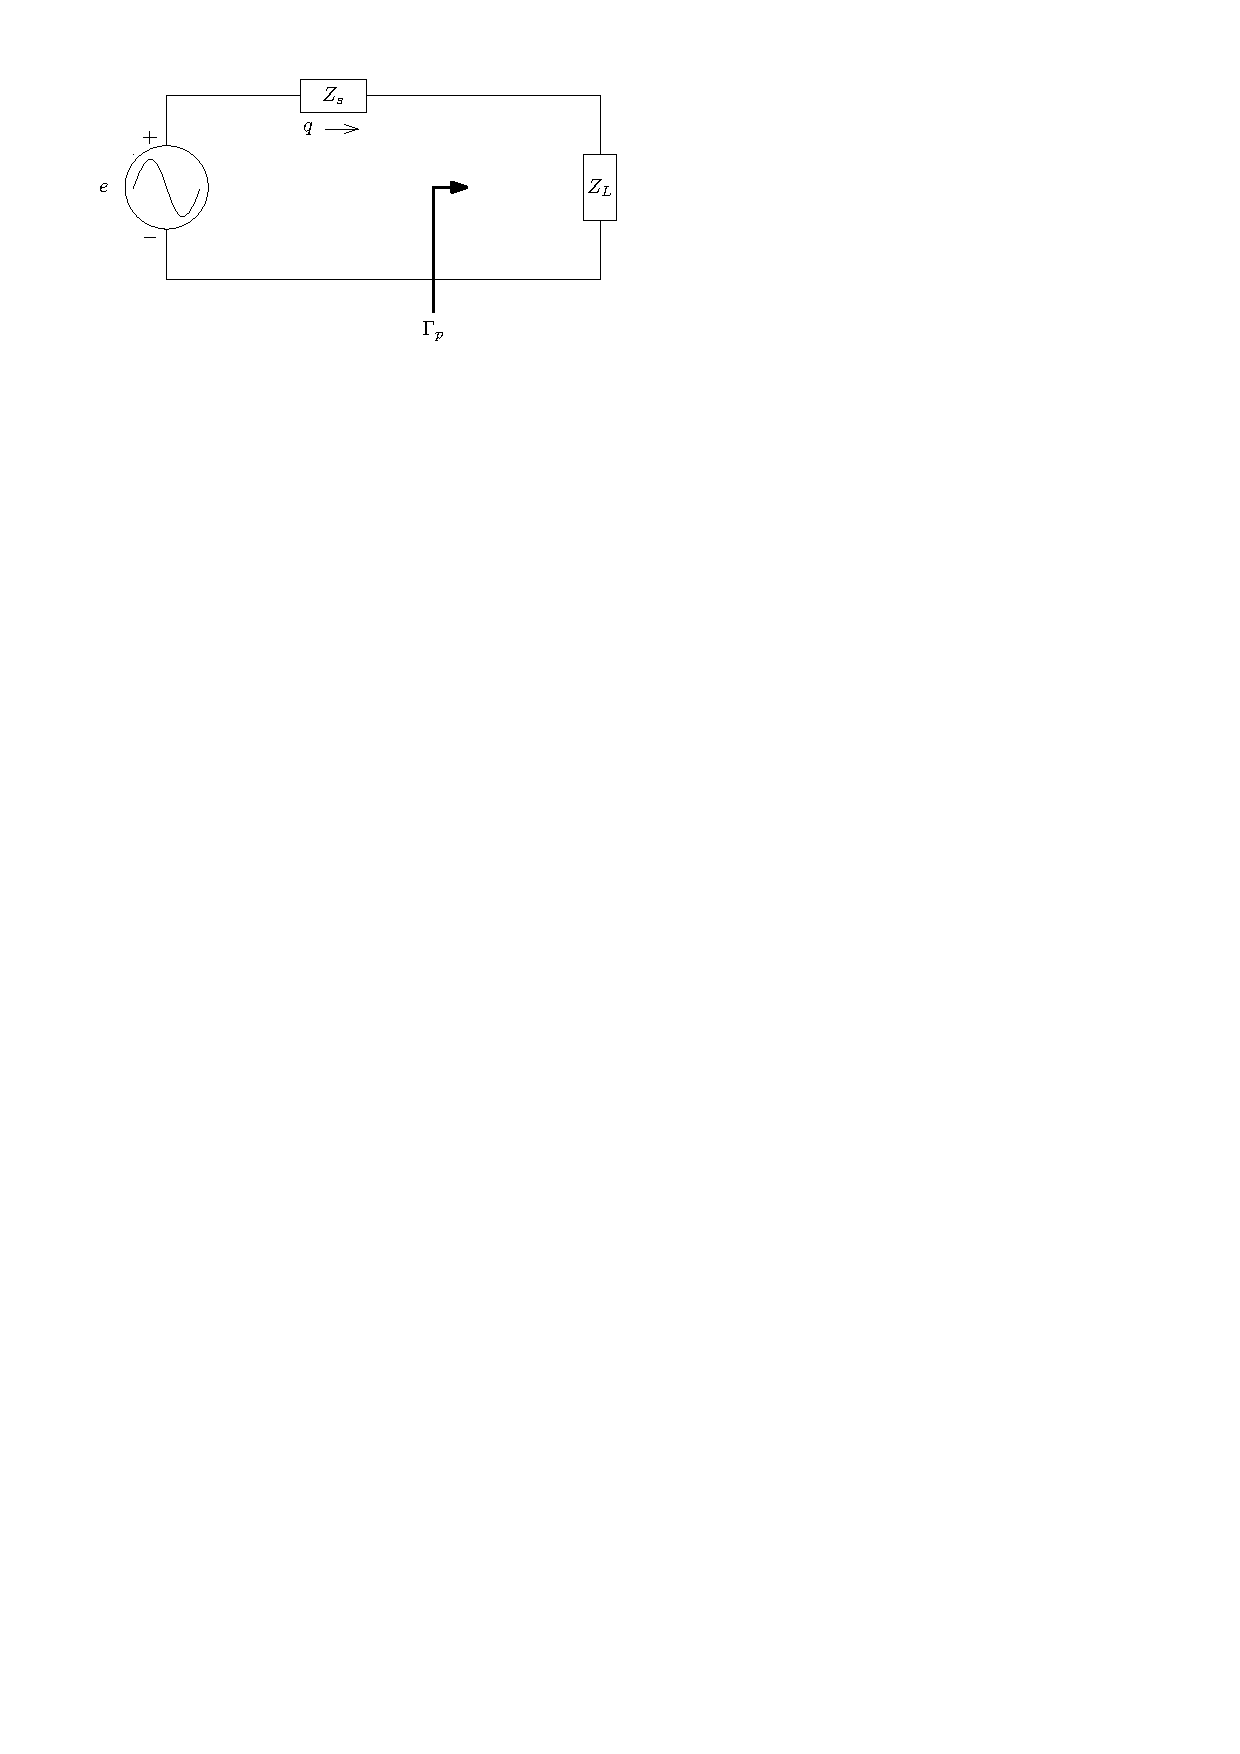
\includegraphics[width=1\columnwidth]{wec_as_multiport_reflection_coefficient.pdf}
        \caption{Power reflection coefficient ($\Gamma$) in a simple system looking from the source impedance ($Z_s$) towards the load impedance ($Z_L$).}
        \label{fig:wec_as_multiport_reflection_coefficient}
\end{figure}
%
\begin{equation}
        \Gamma =\left| \frac{Z_L - Z_s^*}{Z_L + Z_s} \right|^2
        \label{eq:reflection_coeff_impedances}
\end{equation}
%
Note that the fraction of power transmitted (the ``power transmission coefficient'') is $1 - \Gamma$.
We can see from \eqref{eq:reflection_coeff_impedances} that when the matching condition $Z_L = Z_s^*$ is satisfied, $\Gamma$ will be zero and all power will be transmitted.
Note that we may calculate reflection/transmission coefficients at different points within the system (consider, e.g., \figurename~\ref{fig:wec_as_multiport_circuits}e, where we may examine power reflection/transmission at the input of the PTO by comparing $Z_{\textrm{in}}$ and $Z_i$).

% ------------------------------------------------------------------
\section{Illustrative examples}\label{sec:illustrative_examples}
Many problems in WEC design can be examined through the concepts discussed in Section~\ref{sec:modeling_a_direct_drive_wec}.
We will consider a subset of these applications in the subsequent sections.%
% \footnote{Source code to reproduce these results is available at \url{https://github.com/ryancoe/wec_as_multiport}} XX

% ------------------------------------------------------------------
\subsection{Control design}\label{sec:control_design}
One very relevant and illustrative case is a scenario in which the machine design is assumed fixed, and we must maximize performance by setting the load impedance (i.e., by designing a controller).
Many papers in the area of WEC control have focused on this very problem.
In most cases, those papers consider mechanical power ($\mathcal{S}_{m}$) as the overall problem objective.
%
\begin{equation}
\begin{aligned}
        \mathcal{S}_{m}  &= \frac{1}{2} F_{\textrm{pto}} v^*  = \frac{1}{2}Z_{\textrm{in}} v v^* = \frac{1}{2}Z_{\textrm{in}} | v |^2 \\
        &= \frac{1}{2} Z_{\textrm{in}} \left| \frac{F_{\textrm{exc}}}{Z_i + Z_{\textrm{in}}} \right|^2
\end{aligned}
\end{equation}
%
As discussed in Section~\ref{sec:introduction}, the WEC control design problem is often defined to maximize mechanical power by satisfying impedance matching at the input of the PTO per \eqref{eq:bi_conj_matching_in}.
This disregards the rest of the system and invites possibly deleterious effects, as illustrated in \figurename~\ref{fig:wec_as_multiport_load_impedance_for_mech_power}, which shows the resulting load impedances for two cases:

\begin{itemize}
        \item Controller to maximize \emph{mechanical} power: $C \vert_{Z_{\textrm{in}} = Z_i^*}$
        \item Controller to maximize \emph{electrical} power: $C \vert_{Z_\ell = Z_{\mathrm{out}}^*}$
\end{itemize}%
%
\begin{figure}[tb]
        \centering
        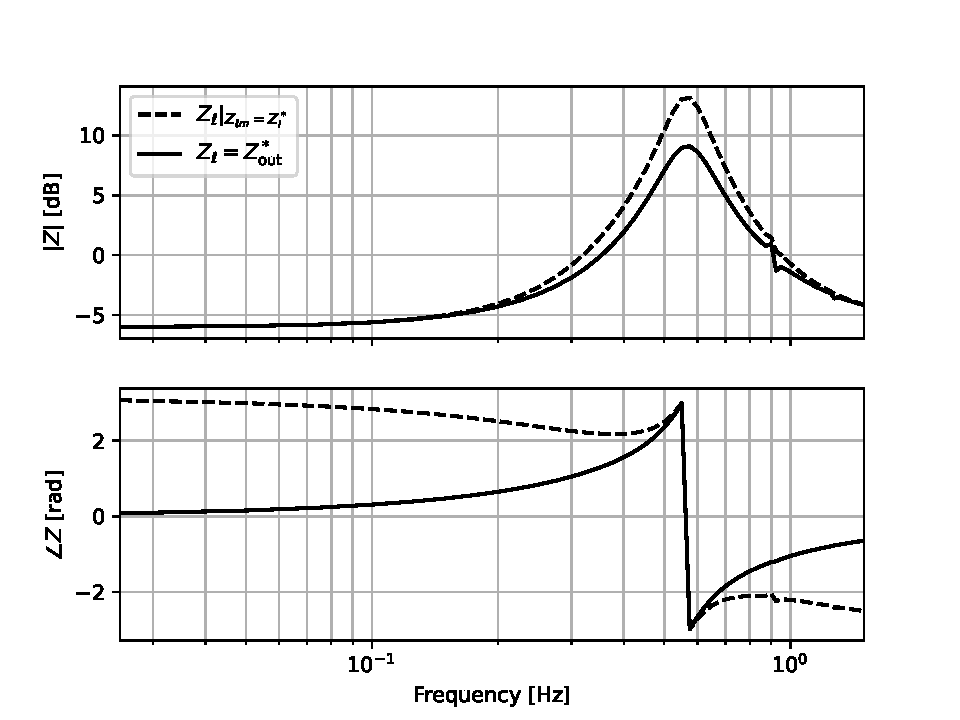
\includegraphics[width=1\columnwidth]{wec_as_multiport_load_impedance_for_mech_power_Bode.pdf}
        \caption{Load impedances (top and middle axes) created by a controller designed to maximize mechanical power ($C \vert_{Z_{\textrm{in}} = Z_i^*}$) and a controller designed to maximize electrical power ($C \vert_{Z_\ell = Z_{\mathrm{out}}^*}$) along with the transducer gains (bottom axes) for each controller.}
        \label{fig:wec_as_multiport_load_impedance_for_mech_power}
\end{figure}
%
From \figurename~\ref{fig:wec_as_multiport_load_impedance_for_mech_power}, we can see that the mechanical power maximizing controller load impedance is notably different from that of the controller that maximizes electrical power.
At $\sim 0.575$\,Hz, both controllers have zero phase, but the magnitudes do not match.
Away from resonance, the phases of the two controllers differ dramatically.
Furthermore, the transducer gain of the two systems is strikingly different, with the gain for the mechanical power maximizing controller \emph{negative} for much of the frequency range -- this means the controller designed to \emph{maximize} mechanical power actually \emph{consumes} electrical power.

The results in \figurename~\ref{fig:wec_as_multiport_load_impedance_for_mech_power} use theoretical optimal controllers.
While higher-order controllers can \emph{approach} a perfect realization of the optimal load impedance per \eqref{eq:bi_conj_matching_out}, perfect matching at all frequencies cannot be achieved in practice.\footnote{Per the Bode-Fano limit, impedance matching can be achieved over only a finite bandwidth -- the limit for the matching bandwidth is proportional to the ratio of resistance to reactance in the impedance.}
However, as noted in \cite{Coe2020a}, real ocean sea states have relatively narrow bandwidths, meaning that a given controller only needs to match the load impedance over a narrow frequency range -- the controller can be updated to accommodate changing sea states \cite{Forbush:2022aa}.
These concepts are illustrated in \figurename~\ref{fig:gfx/wec_as_multiport_pi_controllers_real_imag}, where PI controllers are tuned for waves with frequencies 0.4, 0.55, and 0.65\,Hz.
While the three controllers each achieve perfect impedance matching at only a single frequency, we can see from the transducer gain that they perform quite well relative to the theoretical optimal over a limited frequency range.

\begin{figure}[tb]
        \centering
        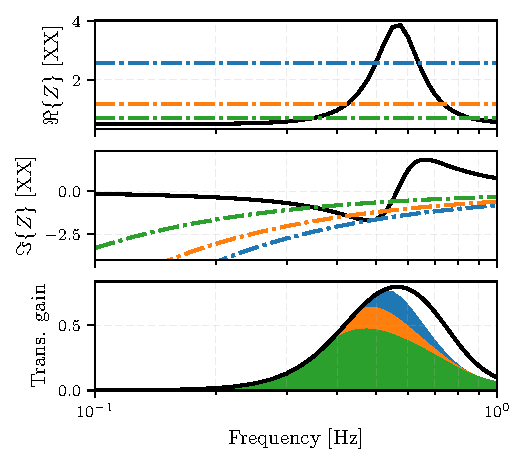
\includegraphics[width=1\columnwidth]{wec_as_multiport_pi_controllers_real_imag.pdf}
        \caption{Optimal load impedance (black curve) and load impedances produced by three PI controllers (colored curves) tuned for different design frequencies (dashed vertical lines; $f_d = [0.4, 0.55, 0.65]$\,Hz) with corresponding transducer gains.}
        \label{fig:gfx/wec_as_multiport_pi_controllers_real_imag}
\end{figure}

% ------------------------------------------------------------------
\subsection{PTO co-design}\label{sec:pto_codesign}
From \eqref{eq:bi_conj_matching}, we can see clear guidance for how the machine and controller can be designed to maximize power delivered to the load (i.e., maximize electrical power output).
Consider, for example, \figurename~\ref{fig:wec_as_multiport_in_and_out_impedances}, where we separately investigate the effects of adding a negative stiffness element\footnote{The addition of a negative stiffness element has been applied in WEC design by CorPower in the form of a hydraulic assembly \cite{Todalshaug:2016aa} and also by Sandia Labs via a tunable magnetic spring \cite{Forbush:2024aa}.} to the drive-train (\figurename~\ref{fig:wec_as_multiport_in_and_out_impedances_spring}) and adding inertia to the drive-train (\figurename~\ref{fig:wec_as_multiport_in_and_out_impedances_inertia}).
The left-hand axes in each figure show $Z_{\textrm{in}}$ (colored curves) along with $Z_i^*$ (black dashed curve), which we are essentially attempting to match by altering the machine design.
The right-hand axes in each figure show $Z_{\textrm{out}}$.
In each case, we enforce \eqref{eq:bi_conj_matching_out} such that the theoretical optimal load impedance ($Z_\ell$) is used to maximize electrical power.

\begin{figure}
     \centering
     \begin{subfigure}[b]{1\columnwidth}
         \centering
         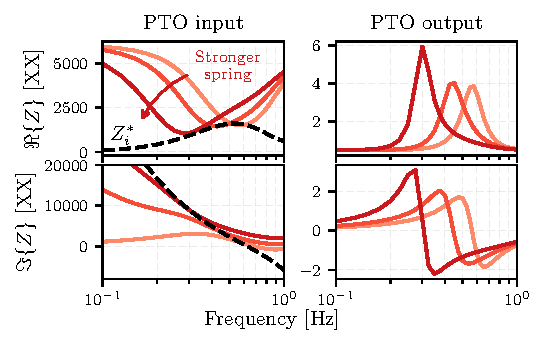
\includegraphics[width=\textwidth]{wec_as_multiport_in_and_out_impedances_spring.pdf}
         \caption{Varying levels of stiffness on shaft ($K_d=[0, -50, -100]$\,Nm/rad)}
         \label{fig:wec_as_multiport_in_and_out_impedances_spring}
     \end{subfigure}
     \\
     \begin{subfigure}[b]{1\columnwidth}
         \centering
         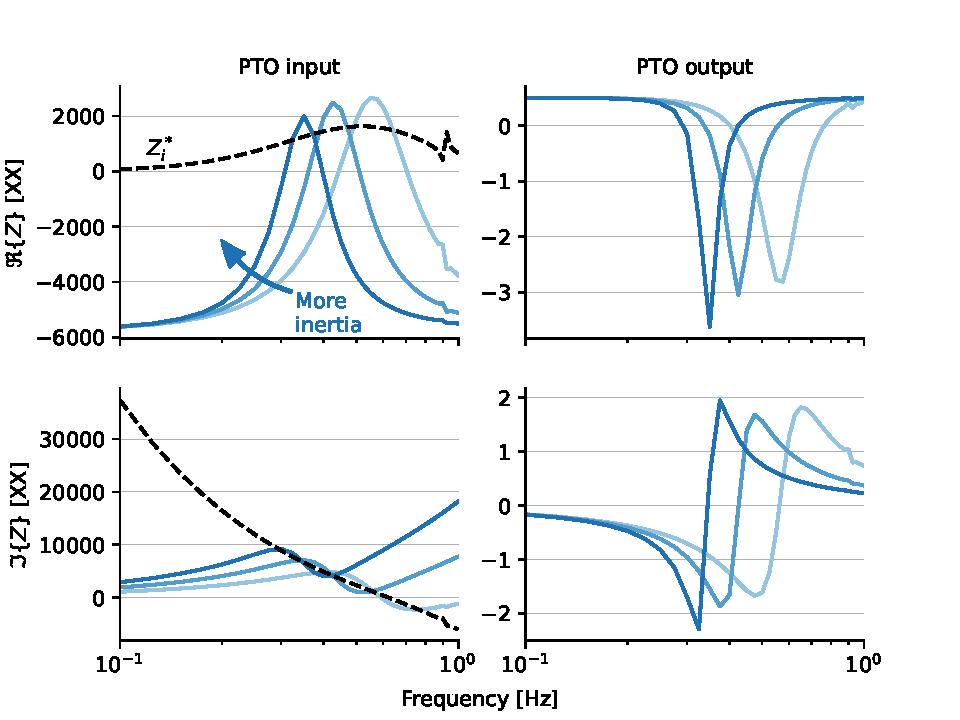
\includegraphics[width=\textwidth]{wec_as_multiport_in_and_out_impedances_inertia.pdf}
         \caption{Varying levels of shaft inertia ($I_d=[2, 11, 20]$\,kg m$^2$)}
         \label{fig:wec_as_multiport_in_and_out_impedances_inertia}
     \end{subfigure}
     \caption{Input port (left) and output port (right) impedances. Upper axes show real part ($\Re \{ Z \}$), lower axes show imaginary part ($\Im \{ Z \}$). Impedance matching condition on the input port per \eqref{eq:bi_conj_matching_in} illustrated by black dashed curve.}
     \label{fig:wec_as_multiport_in_and_out_impedances}
\end{figure}

Both of the considered design alterations (negative stiffness and increased shaft inertia) have the effect of improving impedance matching on the input port at lower frequencies.
Recall also that the power transported by an ocean wave is inversely proportional to the wave frequency ($J \propto f^{-1}$) and that lower frequency (longer wavelength) waves can grow to larger amplitudes before breaking, meaning that this improved impedance matching at lower frequencies may be particularly advantageous.
It should be noted that the range of values for $K_d$ and $J_d$ shown in \figurename~\ref{fig:wec_as_multiport_in_and_out_impedances} is somewhat arbitrary and intended only to illustrate trends -- one cannot directly compare the effects of doubling the shaft inertia with doubling the negative spring stiffness in terms of an engineering decision.
With this in mind, we can see that, for this specific example, adding shaft inertia (\figurename~\ref{fig:wec_as_multiport_in_and_out_impedances_inertia}) appears to adversely affect the shape of the input impedance (both in terms of the real and imaginary parts) by narrowing the bandwidth over which a good matching with the intrinsic impedance is achieved, whereas adding a negative spring (\figurename~\ref{fig:wec_as_multiport_in_and_out_impedances_spring}) appears to have the opposite effect, generally increasing the bandwidth over which good matching with the intrinsic impedance occurs.
While we might intuitively expect that changes to $K_d$ and $J_d$ would only affect the imaginary part of the impedances, we can see from \eqref{eq:expanded_z} that these terms do indeed affect the real part of the impedances as well.

The resulting performance of these different designs can be characterized using the power reflection coefficient in \eqref{eq:reflection_coeff_impedances}.
The power reflection coefficient is an appropriate tool to compare these design strategies as they alter the input impedance of the PTO, XX
\figurename~\ref{wec_as_multiport_spring_inertia_power_reflection_coefficient} shows the power reflection coefficient at the input of the PTO 
As noted from \figurename~\ref{fig:wec_as_multiport_in_and_out_impedances}, the negative spring creates a broader impedance matching, and thus we observe a broader range of very low power reflection at the input of the PTO in the spring designs than in the shaft inertia designs.

\begin{figure}[tb]
        \centering
        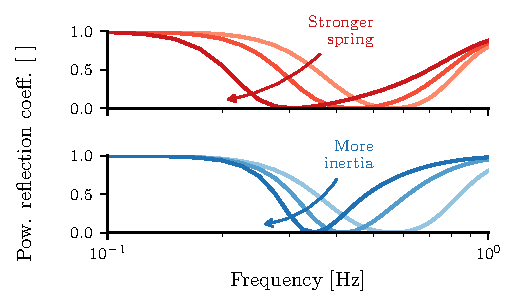
\includegraphics[width=1\columnwidth]{wec_as_multiport_spring_inertia_power_reflection_coefficient.pdf}
        \caption{Power take-off input power reflection coefficients for different levels of spring stiffness (top axes with red curves; $K_d=[0, -50, -100]$\,Nm/rad) and shaft inertia (bottom axes with blue curves; $I_d=[2, 11, 20]$\,kg\,m$^2$).}
        \label{wec_as_multiport_spring_inertia_power_reflection_coefficient}
\end{figure}

Of course, we do not need to apply these design strategies exclusively, and in practice we would consider altering the shaft inertia and negative spring together, along with many other design parameters.
Different WEC archetypes will have different design parameters that can be considered through this same lens.
For example, an oscillating water column design could consider the shaft inertia, air chamber volume (related to stiffness), and many other factors.
The inertia and restoring stiffness of a flap device, along with other properties, will be strongly tied to the height of the flap and its ballasting.

% ------------------------------------------------------------------
\section{Discussion and conclusions}
Expanding on \cite{Bacelli:2021aa}, this paper casts WEC design as an impedance shaping problem.
Sizing/shaping the hull, altering the drive-train, motor/generator selection, control design, and many more factors all have interrelated effects on the impedance matching and therefore on the power delivered to the load.
In practice, the bi-conjugate impedance matching requirement expressed by \eqref{eq:bi_conj_matching} cannot be perfectly satisfied at all frequencies, and the cost of improving the matching condition must be balanced with the resulting benefits.
Furthermore, this formulation does not capture constraints (e.g., maximum torque from a generator or maximum travel of a linear piston) and nonlinear dynamics, which eventually must be considered.
Given these practical considerations, numerical optimization becomes a useful tool.
Nonetheless, the linear modeling approach presented here provides a critical starting point and foundation to build from.

% ------------------------------------------------------------------
\section{Acknowledgements}
The authors would like to acknowledge funding support from the US Department of Energy's Water Power Technologies Office.
Sandia National Laboratories is a multi-mission laboratory managed and operated by National Technology and Engineering Solutions of Sandia, LLC., a wholly owned subsidiary of Honeywell International, Inc., for the U.S. Department of Energy's National Nuclear Security Administration under contract DE-NA0003525.
This paper describes objective technical results and analysis.
Any subjective views or opinions that might be expressed in the paper do not necessarily represent the views of the U.S. Department of Energy or the United States Government.

% ------------------------------------------------------------------
\bibliographystyle{plain}
\bibliography{wec_as_multiport.bib}

\end{document}
